\documentclass[12pt]{beamer}

\usetheme{Air}
\usepackage{thumbpdf}
\usepackage{wasysym}
\usepackage{ucs}
\usepackage[utf8]{inputenc}
\usepackage{pgf,pgfarrows,pgfnodes,pgfautomata,pgfheaps,pgfshade}
\usepackage{verbatim}

\usepackage{gitinfo2}
\usepackage{tikz}
\usepackage{subfig}

\usepackage[absolute,overlay]{textpos}
\usepackage{graphicx}

\usetikzlibrary{fadings}
\usetikzlibrary{positioning}
\usetikzlibrary{arrows, matrix}

\makeatletter
\newbox\@backgroundblock
\newenvironment{backgroundblock}[2]{%
  \global\setbox\@backgroundblock=\vbox\bgroup%
    \unvbox\@backgroundblock%
    \vbox to0pt\bgroup\vskip#2\hbox to0pt\bgroup\hskip#1\relax%
}{\egroup\egroup\egroup}
\addtobeamertemplate{background}{\box\@backgroundblock}{}
\makeatother



\pdfinfo
{
  /Title       (What limits fire, where and when?)
  /Creator     (CEH)
  /Author      (Douglas Kelley - douglas.i.kelley@gmail.com)
}

\title{JULES-INFERNO in the Fire Model Intercomparison Project}
\subtitle{Model performance and development reccomendations}
\author{Douglas Kelley, Stijn Hantson, Stephane Mangeon \newline
        \tiny{FireMIP contributors: Almut Arneth, Sandy P. Harrison, Sam S. Rabin, Dominique M. Bachelet, Matthew Forrest, Silvia Kloster, Gitta Lasslop, Fang Li, Joe R. Melton, Tim Sheehan, Chao Yue} \newline
        \tiny{Fire Limitation Framework: Ioannis Bistinas, Rhys Whitley, Chantelle Burton, Toby Marthews}}
\date{\vspace*{-0.6cm}27th June 2017}

\titlegraphic{
\includegraphics[width=2.0cm]{logos/cehlogo945}\hspace*{0.15cm}~%
              
\includegraphics[width=1.5cm]{logos/Met_Office.png}\hspace*{0.2cm}~%
              
\includegraphics[width=1.5cm]{logos/ukesm-logo}\hspace*{0.2cm}~%
              
\includegraphics[width=1.5cm]{logos/suncorp.png}\hspace*{0.2cm}~%
              
\includegraphics[width=1.5cm]{logos/VU.png}\hspace*{0.15cm}~%
              
\includegraphics[width=2.0cm]{logos/nerc-long-logo-large}

              %\tiny{url: https://github.com/douglask3/LimFIRE ---
              %      revision no: \gitAbbrevHash}
             }

\begin{document}

\frame{\titlepage}
\title{JULES-INFERNO in fireMIP}

\author{Douglas Kelley, Stijn Hantson, Stephane Mangeon}

%\section*{}
%\begin{frame}
%  \frametitle{Outline}
%  \tableofcontents[section=1,hidesubsections]
%\end{frame}

%\AtBeginSection[]
{
  \pgfdeclareimage[width=1.0\paperwidth]{header-image}{header_images/fire}
%  \frame<handout:0>
%  {
%    \frametitle{Outline}
%    \tableofcontents[currentsection,hideallsubsections]
%  }
}

%\AtBeginSubsection[]
%{
%  \frame<handout:0>
%  {
%    \frametitle{Outline}
%    \tableofcontents[sectionstyle=show/hide,subsectionstyle=show/shaded/hide]
%  }
%}\textsl{}

\newcommand<>{\highlighton}[1]{%
  \alt#2{\structure{#1}}{{#1}}
}

\newcommand{\icon}[1]{\pgfimage[height=1em]{#1}}


%%%%%%%%%%%%%%%%%%%%%%%%%%%%%%%%%%%%%%%
%%%%%%%%%% Content starts here %%%%%%%%%%
%%%%%%%%%%%%%%%%%%%%%%%%%%%%%%%%%%%%%%%%%

\section{Introduction}
\pgfdeclareimage[width=1.0\paperwidth]{header-image}{header_images/fire2}


% Fire is important - why
% However, changes in fire are uncertain - fireMIP and Gittas paper.
% fireMIP
% JULES model type
% JULES performance
%  - best model of type
%  - best with prescribed veg
%  - veg model evaluation
%  - fire model evaultatrion
% Human fires
% Human suppression
%    From scores
%    From other studies
% Conclusions
% Slide to leave up: Other areas of fireMIP

% Slide 1: Burnt area; Areas of effected plants; Emissions; Radiative forcing
% Slide 2: FireMIP; Gittas model comp; Gittas benchmarking
% Slide 3: Firemip slide

\addtocounter{framenumber}{-1}
\begin{frame}
	\frametitle{Fire In the Earth System}
	\only<1> {\framesubtitle{Carbon Cycle and Radiative Forcing}}
	\only<2-> {\framesubtitle{Areas affected}}
	
	
	\begin{textblock*}{14cm}(-0cm ,1.3cm)
		\begin{tikzpicture}
		\visible<1, 4-> {
			
			\node[anchor=south west,inner sep=0] (image) at (0,0) {
				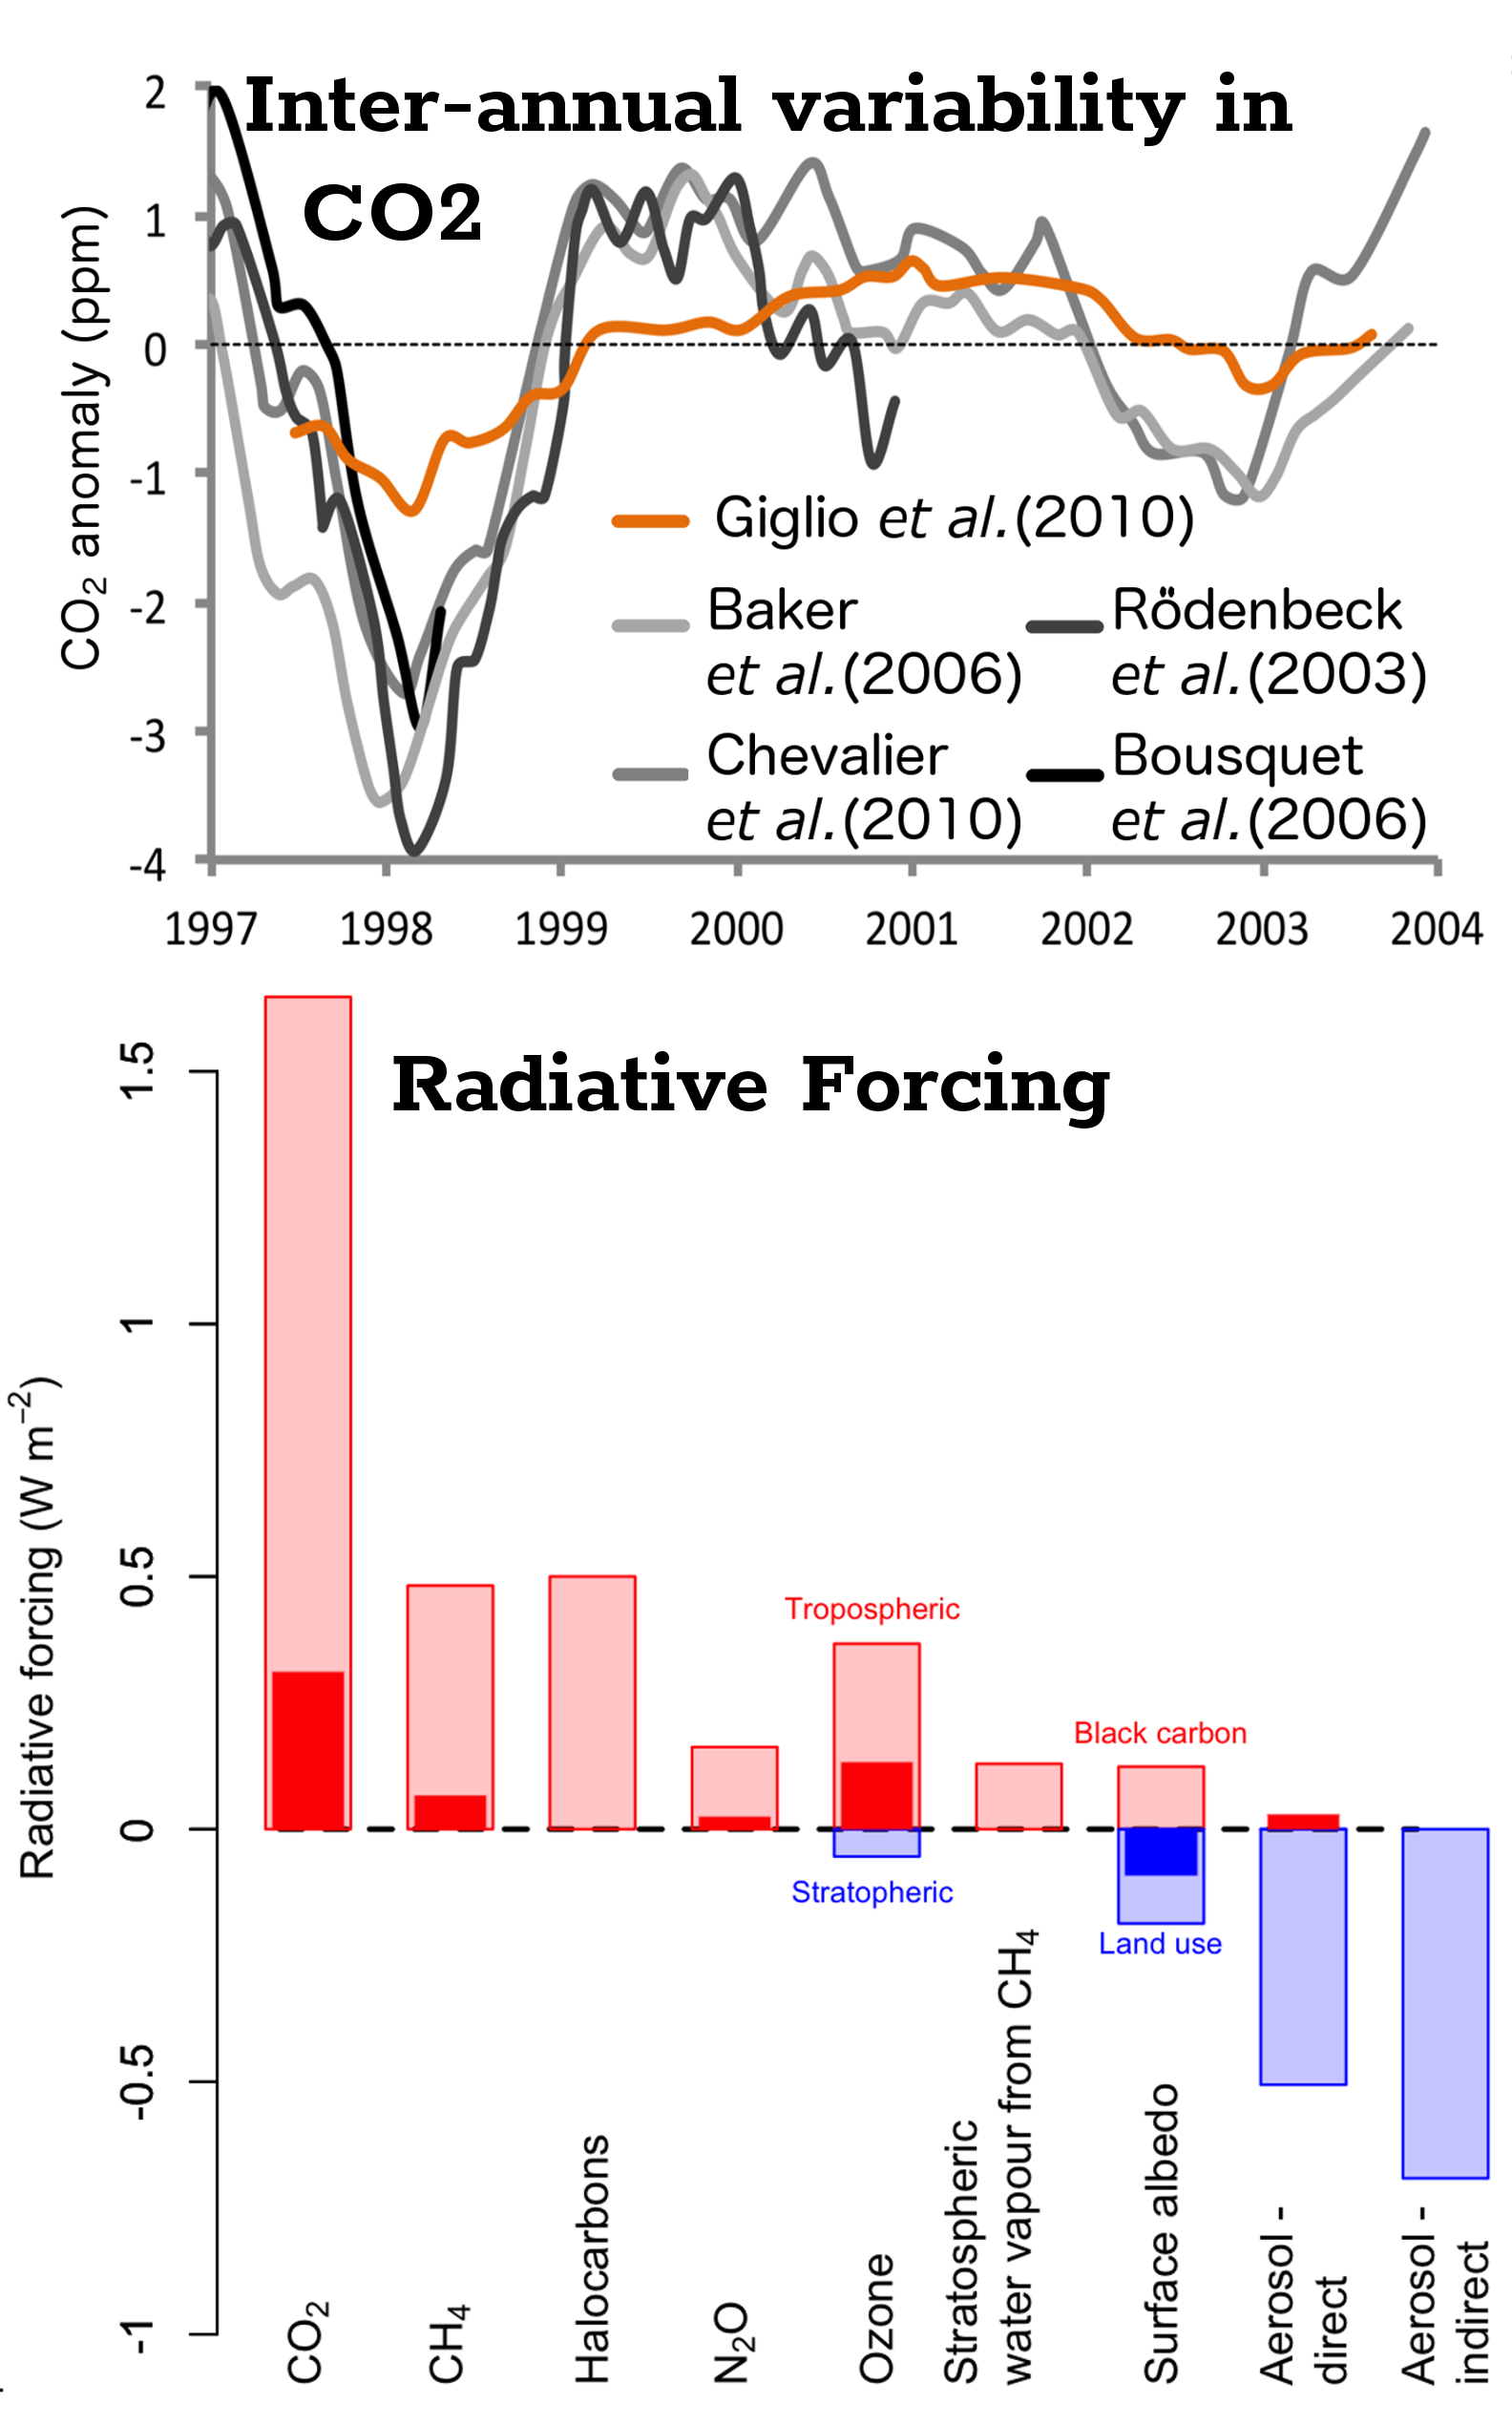
\includegraphics[width=4.80cm]{images/fireImportance}%images/unimodal/p\x.png}
			};}
		
		\only<2-3> {
			\node[anchor=south west,inner sep=0] (image) at (0cm,2cm) {
				\adjincludegraphics[trim={0 {.53\height} 0 0},clip, width=12cm]{images/firePerBiome}%images/unimodal/p\x.png}
			};}
		\only<3>{
				
			\draw[blue, line width = 0.25mm] (5.2,5.65) -- (6.5,5.65) -- (6.5,6) -- (5.2,6) -- (5.2,5.65);
			
			\draw[blue, line width = 0.25mm] (5.6,4.8) -- (6.5,4.8) -- (6.5,5.3) -- (5.6,5.3) -- (5.6,4.8);
			
			\draw[blue, line width = 0.25mm] (9.5,4.5) -- (10.5,4.5) -- (10.5,5.0) -- (9.5,5.0) -- (9.5,4.5);
			
			\draw[blue, line width = 0.25mm] (2.7,4.8) -- (3.5,4.8) -- (3.5,5.3) -- (2.7,5.3) -- (2.7,4.8);
		}		
		
		\visible<4> {
			
			\node[anchor=south west,inner sep=0] (image) at (6.5cm,0cm) {
				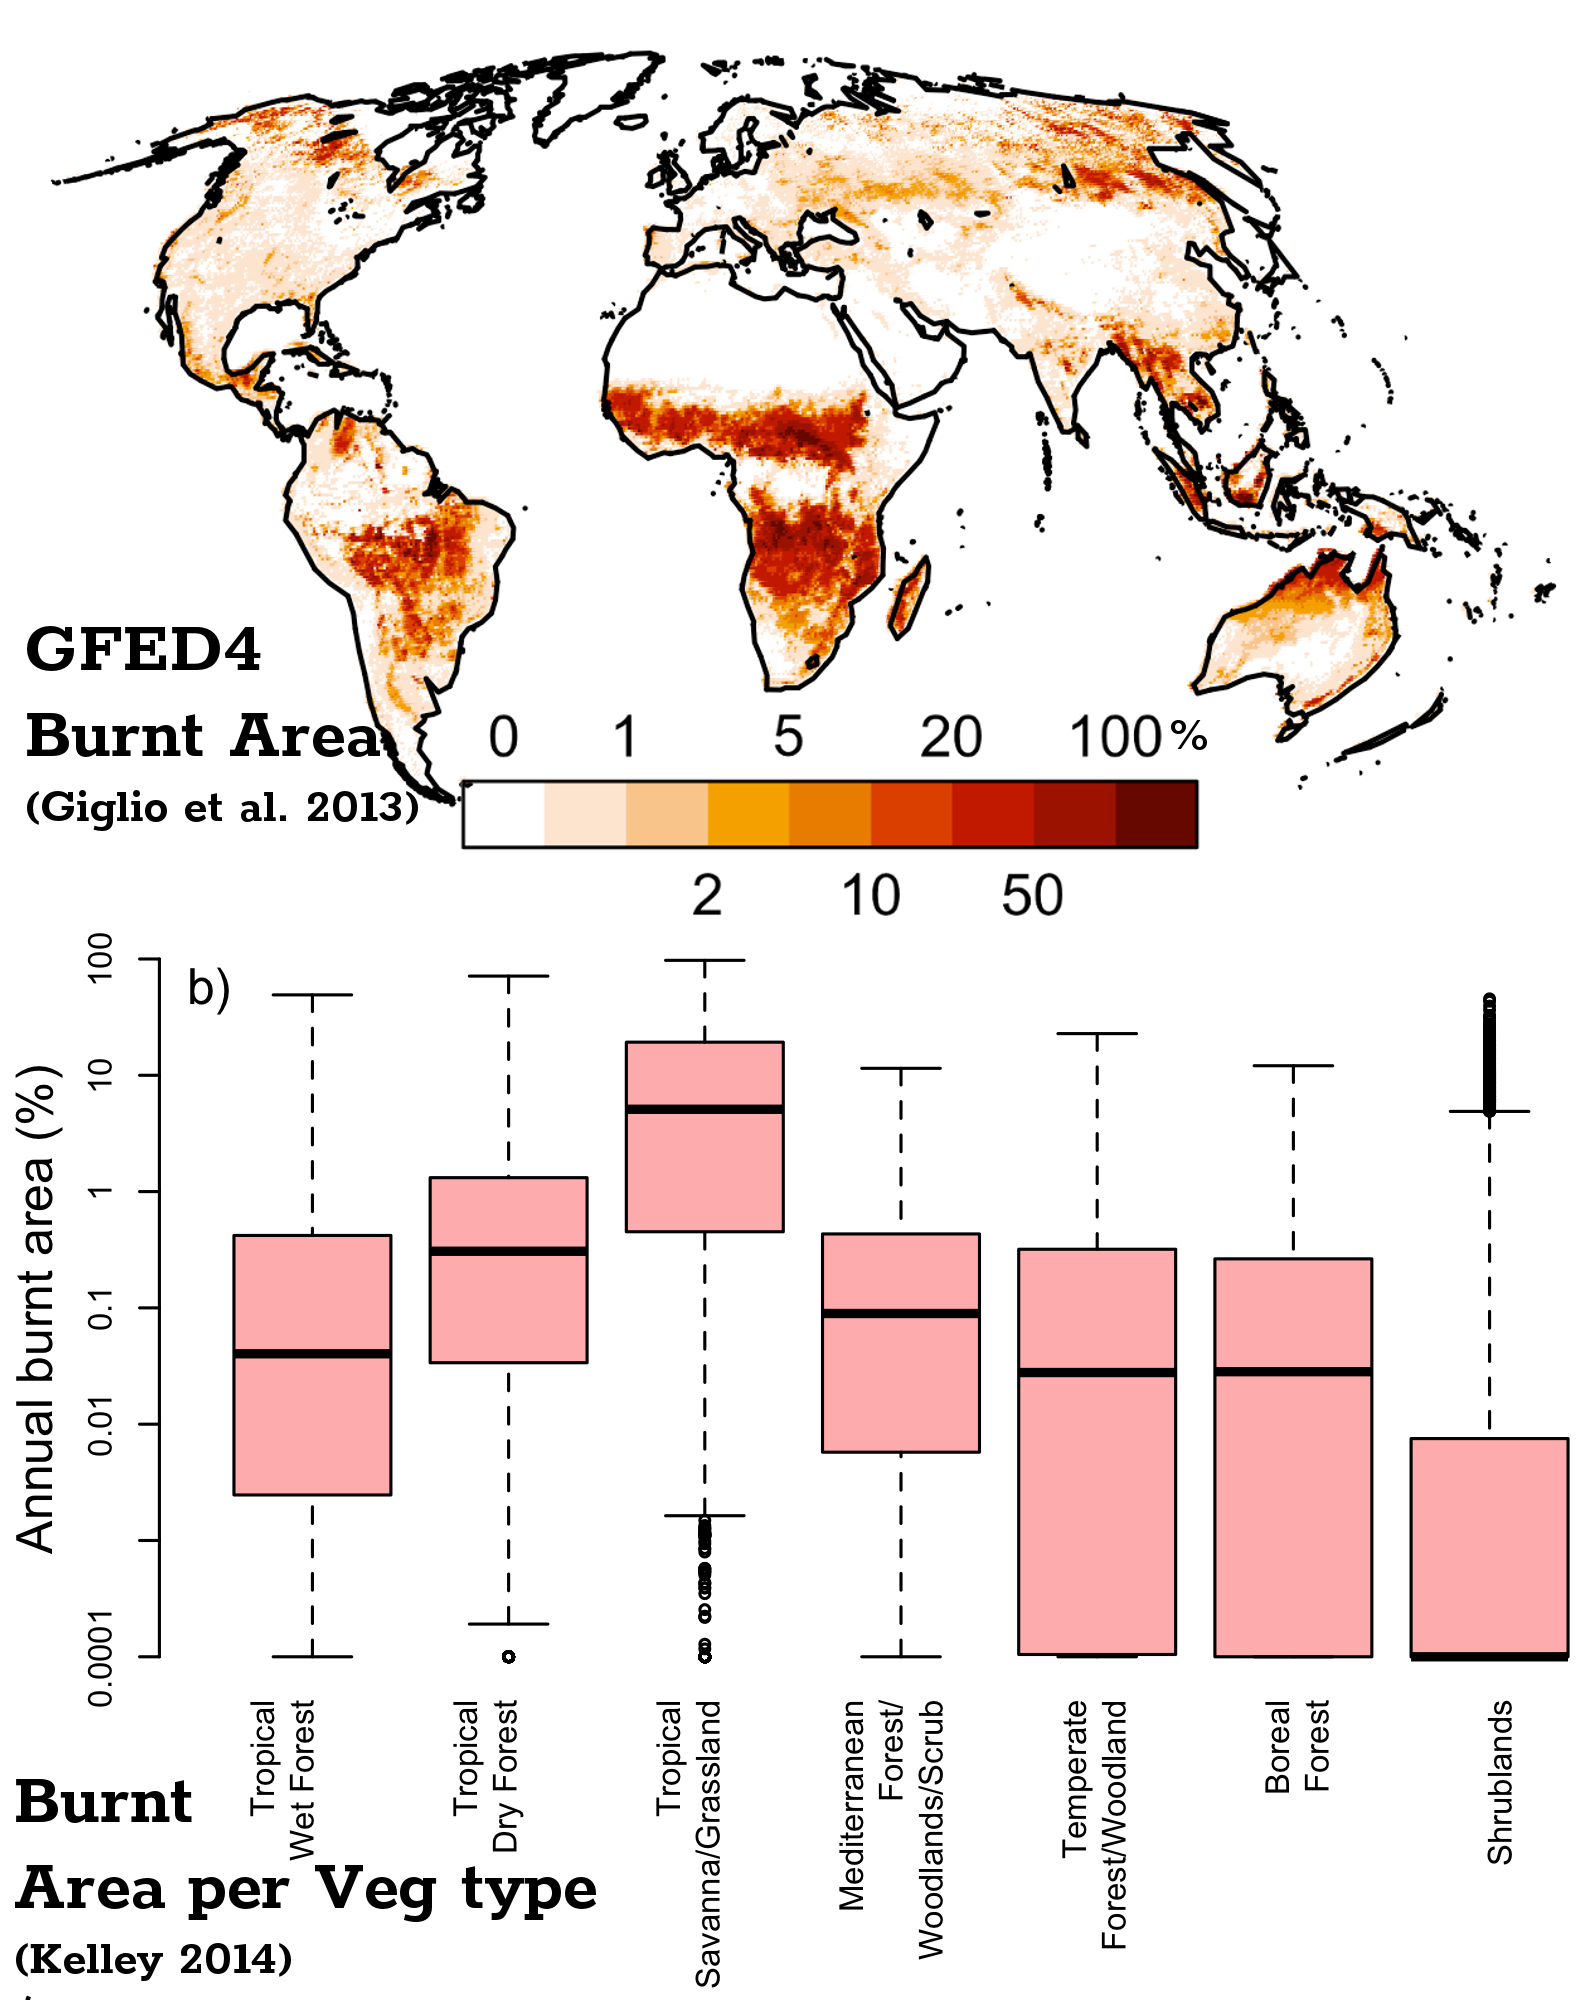
\includegraphics[width=6.05cm]{images/firePerBiome}%images/unimodal/p\x.png}
			};}
		\end{tikzpicture}
	\end{textblock*}
	
	%Make clear we are talking about burnt area
\end{frame}

\begin{frame}[label = intro]
	\frametitle{Fire and carbon}
	%\framesubtitle{Is it Ignitions? Is it people?}
	
	\begin{textblock*}{14cm}(-0cm ,1.3cm)
		\foreach \x in {1, 2, 3, 4, 5, 6, 7, 8, 9} {
			\only<\x> {
				
				\includegraphics[width=10cm]{images/fireCarbonBalance/pp\x.png}
			}
		}
		
	\end{textblock*}
	
	
\end{frame}

\begin{frame}[label = intro]
	\frametitle{fireMIP}
	\framesubtitle{Fire Modelling Inter-comparison Project}
	
	\begin{textblock*}{14cm}(-0.0cm ,1cm)
		%\begin{tikzpicture}
			\foreach \x in {1, 2, 3, 4, 5} {
				\only<\x> {
	%				\node[anchor=south west,inner sep=0] (image) at (0,0) {
						\includegraphics[width=11.7cm]{images/fireMIP/pp\x.png}
	%				};
				}
			}
	\end{textblock*}
	\begin{textblock*}{5.5cm}(7.2cm ,2.5cm)
	%		\node[anchor=south west,inner sep=0] (image) at (6.5cm,0cm) {
				\begin{itemize}
				
					\visible<2->{\item Benchmark overview}
					\visible<3->{\item Focus on JULES performance \& fire controls}
					\visible<4->{\item Diagnose seasonality performance}
					\visible<4->{\item Explore missing anthropogenic processes}
					\visible<5->{\item Other fireMIP evaluation we could take advantage of}
				\end{itemize}
	%		};
	%	\end{tikzpicture}
	\end{textblock*}
			
			%	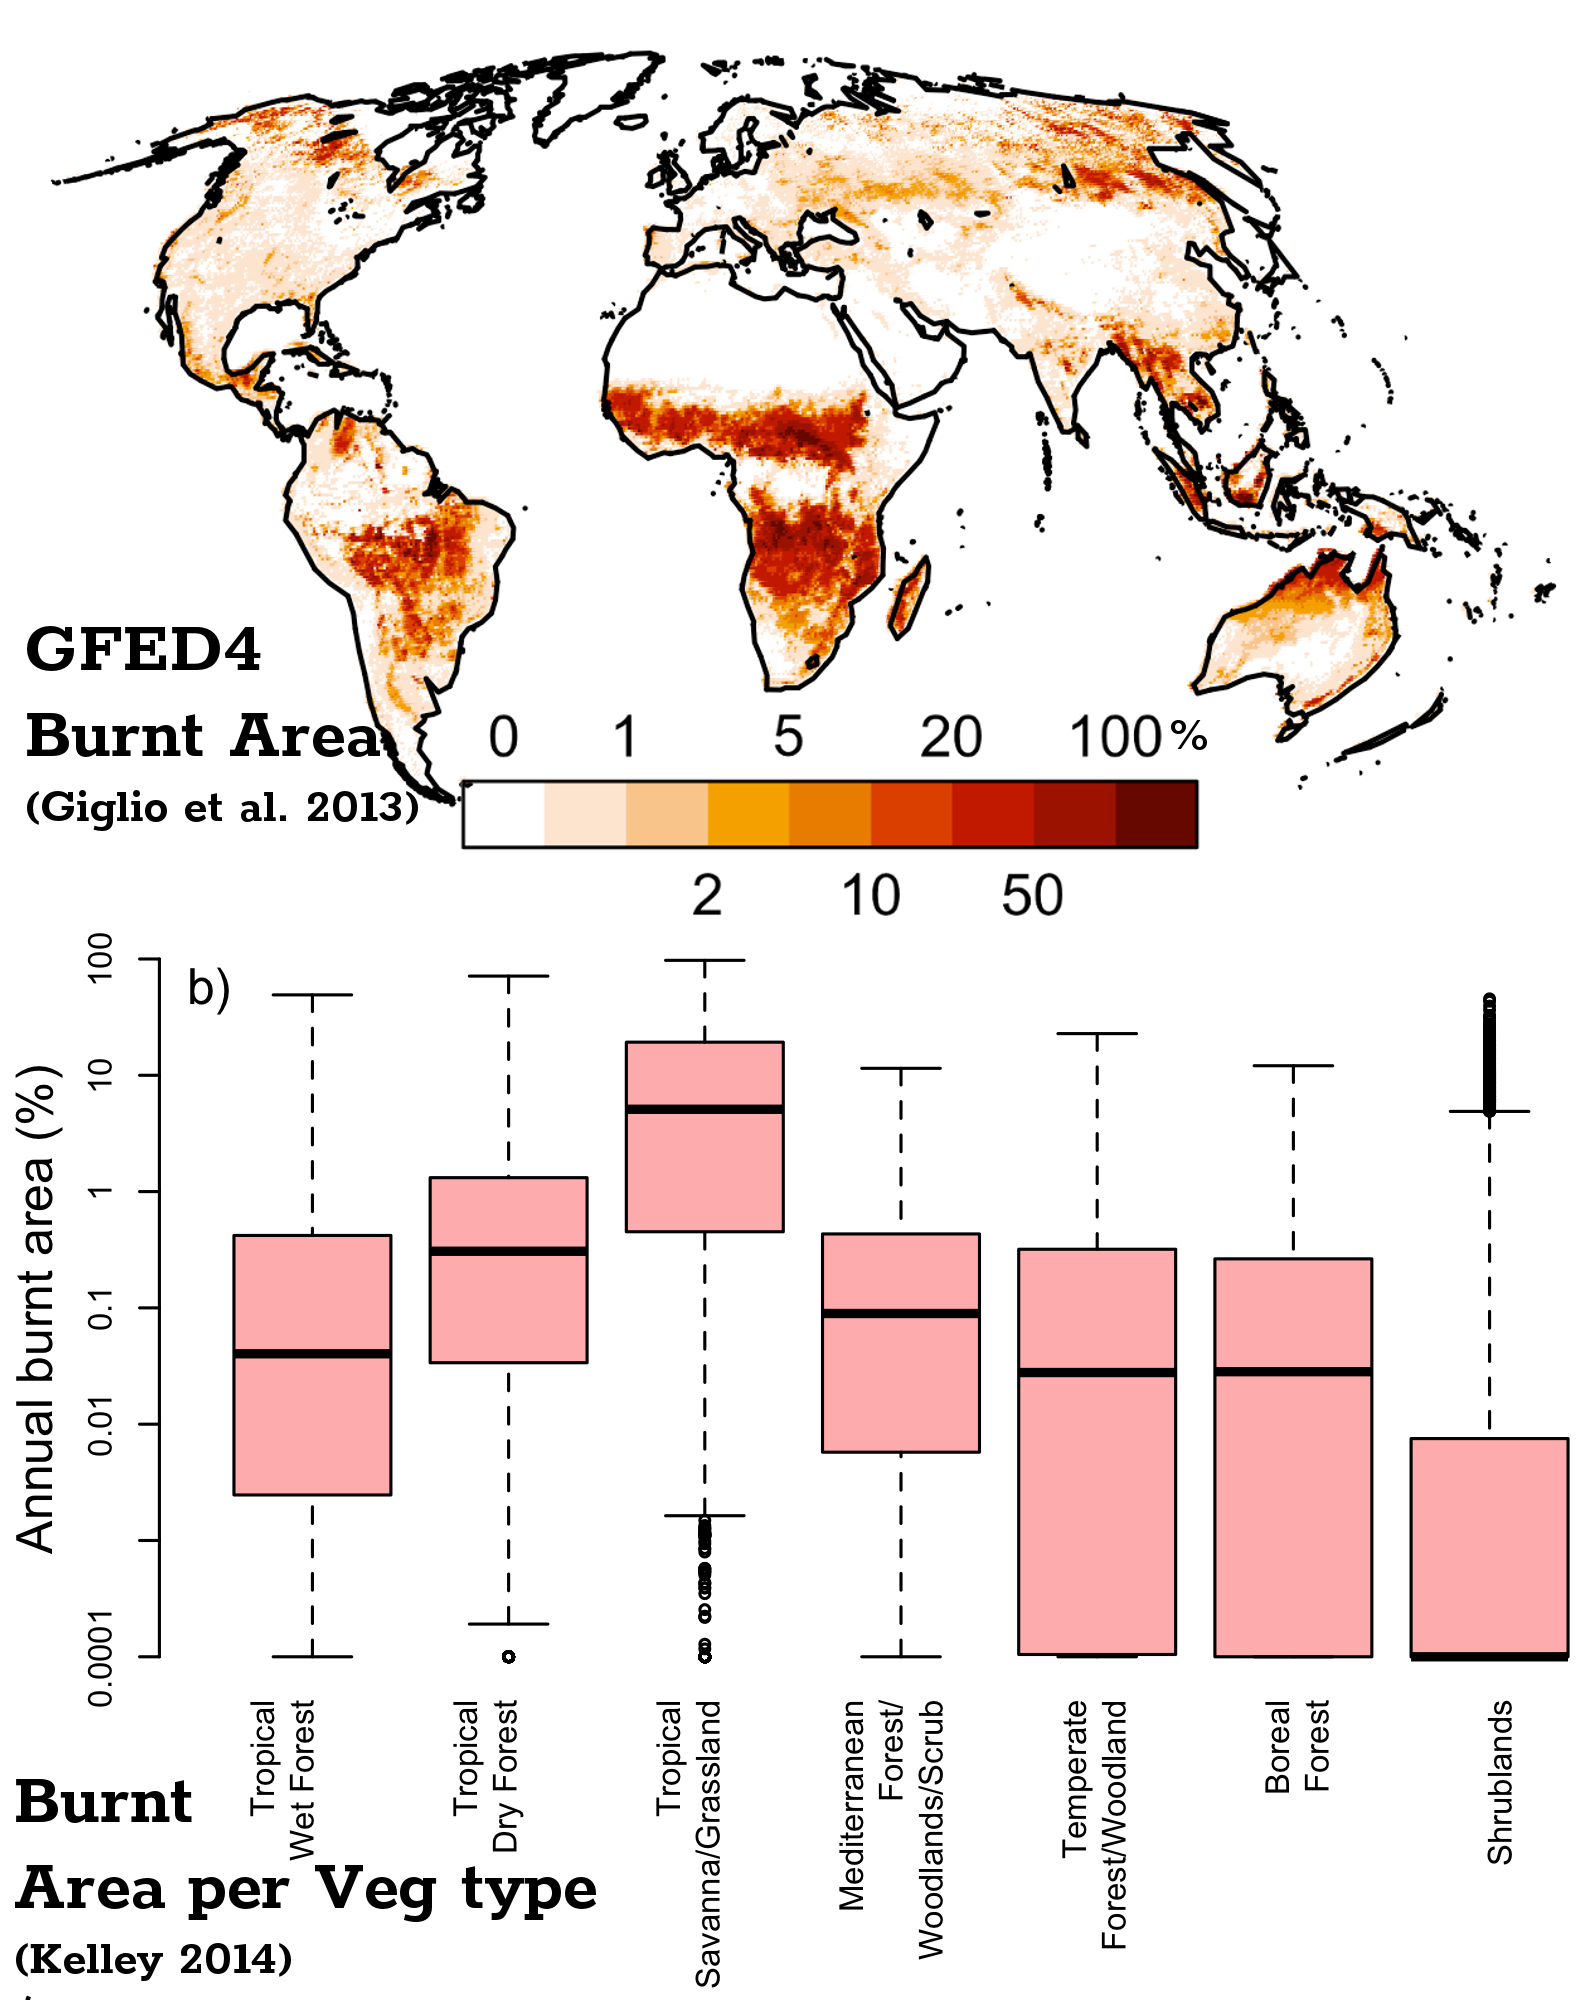
\includegraphics[width=6.05cm]{images/firePerBiome}%images/unimodal/p\x.png}
			%};
	%}}
\end{frame}

%\begin{frame}[label = intro]
%	\frametitle{fireMIP}
%	\framesubtitle{Fire Modelling Inter-comparison Project}
%	\begin{itemize}
%		%\huge{
%			\only<1-4> {
%				\visible<1->{\item Little agreement between models simulated fire}
%				\visible<2->{\item No systematic inter-model comparison of fire or fire drivers}
%				\visible<3->{\item No comparison of different model hindcasts and future projections, and their sensitivity to different drivers}
%				\visible<4->{\item fireMIP setup to address this}
%            }
%	        \only<5-> {
%		        \visible<5->{\item fireMIP model overview}
%		        \visible<6->{\item fireMIP benchmarking system}
%		        \visible<7->{\item Multi-model results}
%		        \visible<8->{\item JULES-INFERNO model performance}
%		        \visible<9->{\item Process evaluation}
%	        }
%	\end{itemize}
%\end{frame}

\section{fireMIP}
\pgfdeclareimage[width=1.0\paperwidth]{header-image}{header_images/red_lightn}

\begin{frame}[label = fireModels]
	\frametitle{fire Models}
	\framesubtitle{Types}
	\foreach \x in {1, 2, 3, 4} {
		\only<\x> {
			\includegraphics[width=10cm]{images/fireModelTypes/pp\x.png}
	}}	
\end{frame}

%\addtocounter{framenumber}{-1}

\begin{frame}[label = kelley2013Datasets]
	\frametitle{FireMIP benchmarking}
	\framesubtitle{Benchmark Datasets}
	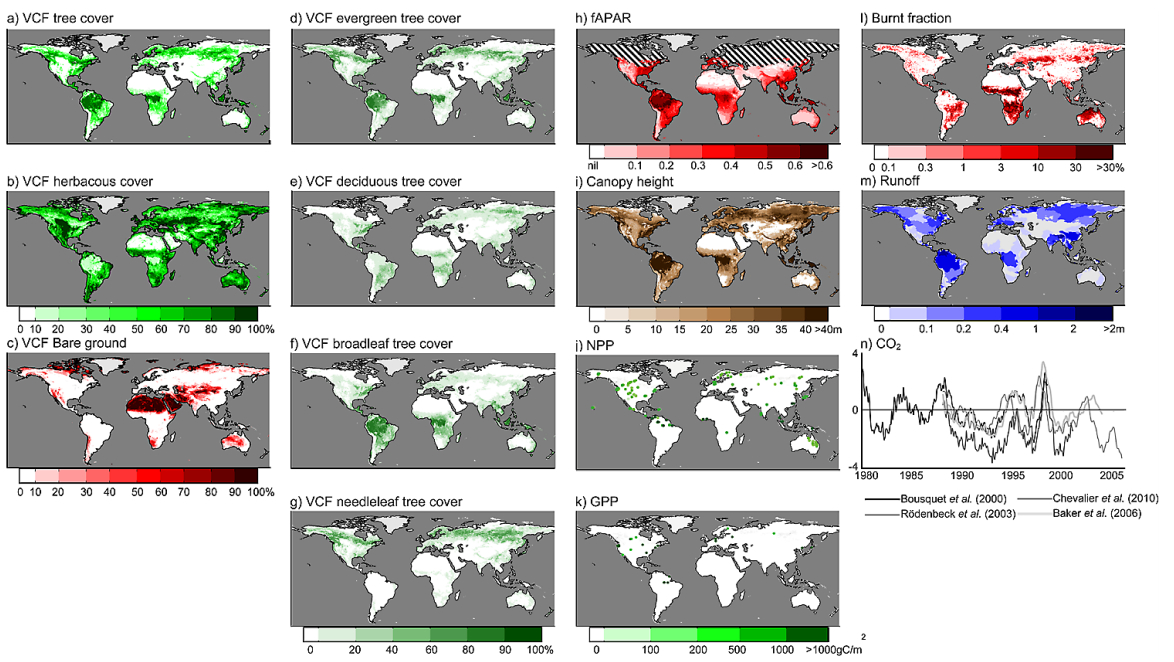
\includegraphics[width=10cm]{images/BenchmarkDatasets.JPG}
	\visible<2-> {
		Plus some new ones
	}
\end{frame}

\addtocounter{framenumber}{-1}

\begin{frame}[label = newDatasets]
	\frametitle{FireMIP benchmarking}
	\framesubtitle{Fire Benchmark Datasets}
	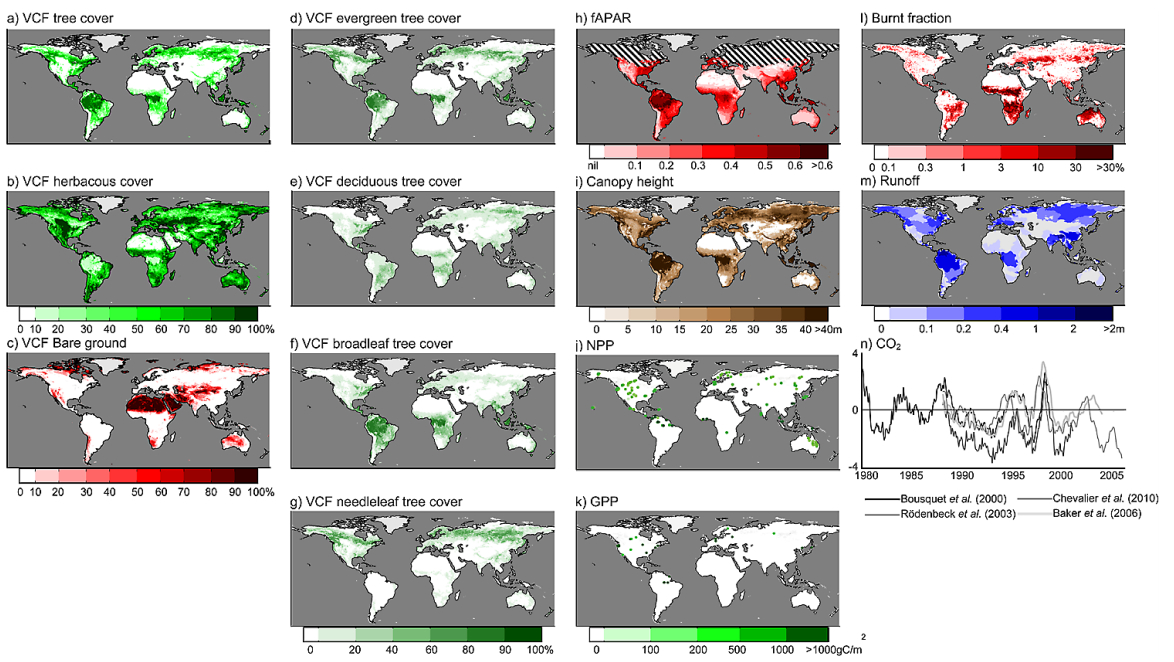
\includegraphics[width=10cm]{images/BenchmarkDatasets.JPG}
\end{frame}

\begin{frame}[label = Metrics]
	\frametitle{FireMIP Metrics}
	\framesubtitle{All Metrics}
	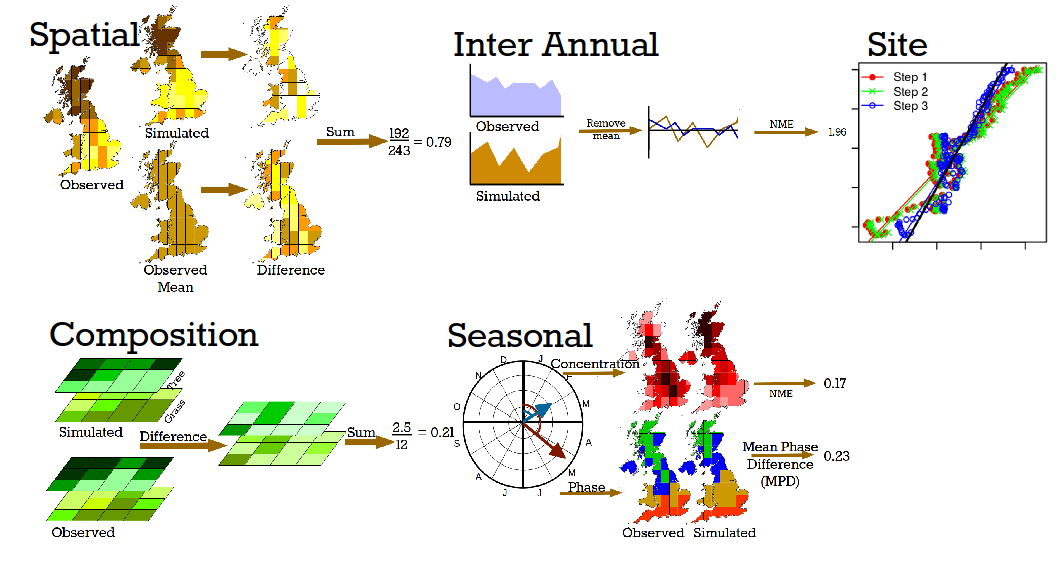
\includegraphics[width=10cm]{images/metrics/Metrics.png}
\end{frame}

\addtocounter{framenumber}{-1}

\begin{frame}[label = MetricsNME]
	\frametitle{FireMIP Metrics}
	\framesubtitle{Normalised Mean Error}
	\foreach \x in {1, 2, 3, 4} {
		\only<\x> {
			\includegraphics[width=10cm]{images/metrics/NME/NME\x.png}
	}}
\end{frame}

\addtocounter{framenumber}{-1}

\begin{frame}<2->[label = MetricsMPD]
	\frametitle{FireMIP Metrics}
	\framesubtitle{Seasonal Comparisons}
	\foreach \x in {1, 2, 3, 4, 5, 6, 7} {
		\only<\x> {
			\includegraphics[width=10cm]{images/metrics/MPD/MPD\x.png}
	}}
\end{frame}

\addtocounter{framenumber}{-1}

\begin{frame}<4>[label = NullModels]
	\frametitle{FireMIP Null Models}
	%\framesubtitle{Seasonal Comparisons}
	\foreach \x in {1,2,3,4} {
		\only<\x> {
			\includegraphics[width=10cm]{images/metrics/NULL/NullModels\x.png}
	}}
\end{frame}

\addtocounter{framenumber}{-1}

\begin{frame}<1-2>[label = Scores]
	\frametitle{FireMIP Null Models}
	%\framesubtitle{Seasonal Comparisons}
	\foreach \x in {1, 2, 3} {
		\only<\x> {
			\includegraphics[width=10cm]{images/metrics/Scores/Scores\x.png}
	}}
\end{frame}
\begin{frame}[label = kelley2013Datasets]
	\frametitle{ Multi-model scores}
	\framesubtitle{Model scores}
	
	% Smileys
	\foreach \x in {1, 2, 3, 4, 5, 6, 7} {
		\only<\x> {
			\includegraphics[width=10cm]{images/modelScores/pp\x.png}
	}}
	%Fire and veg
\end{frame}

\begin{frame}[label = kelley2013Datasets]
	\frametitle{JULES-INFERNO v obs}
	\framesubtitle{Model scores}
	
	\begin{textblock*}{8cm}(11cm ,1.3cm)
		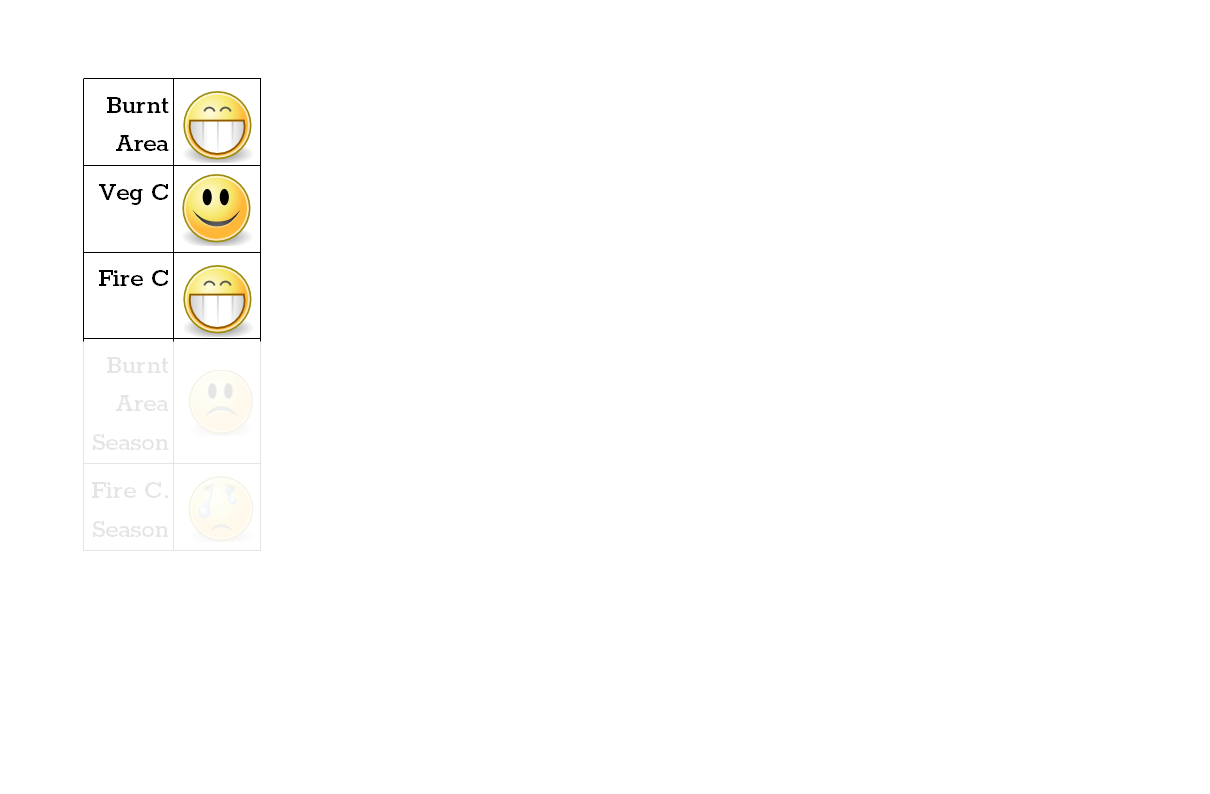
\includegraphics[width=7.5cm]{images/Smileys/BAvegCFireC.png}
	\end{textblock*}
	
	\only<2-> {
		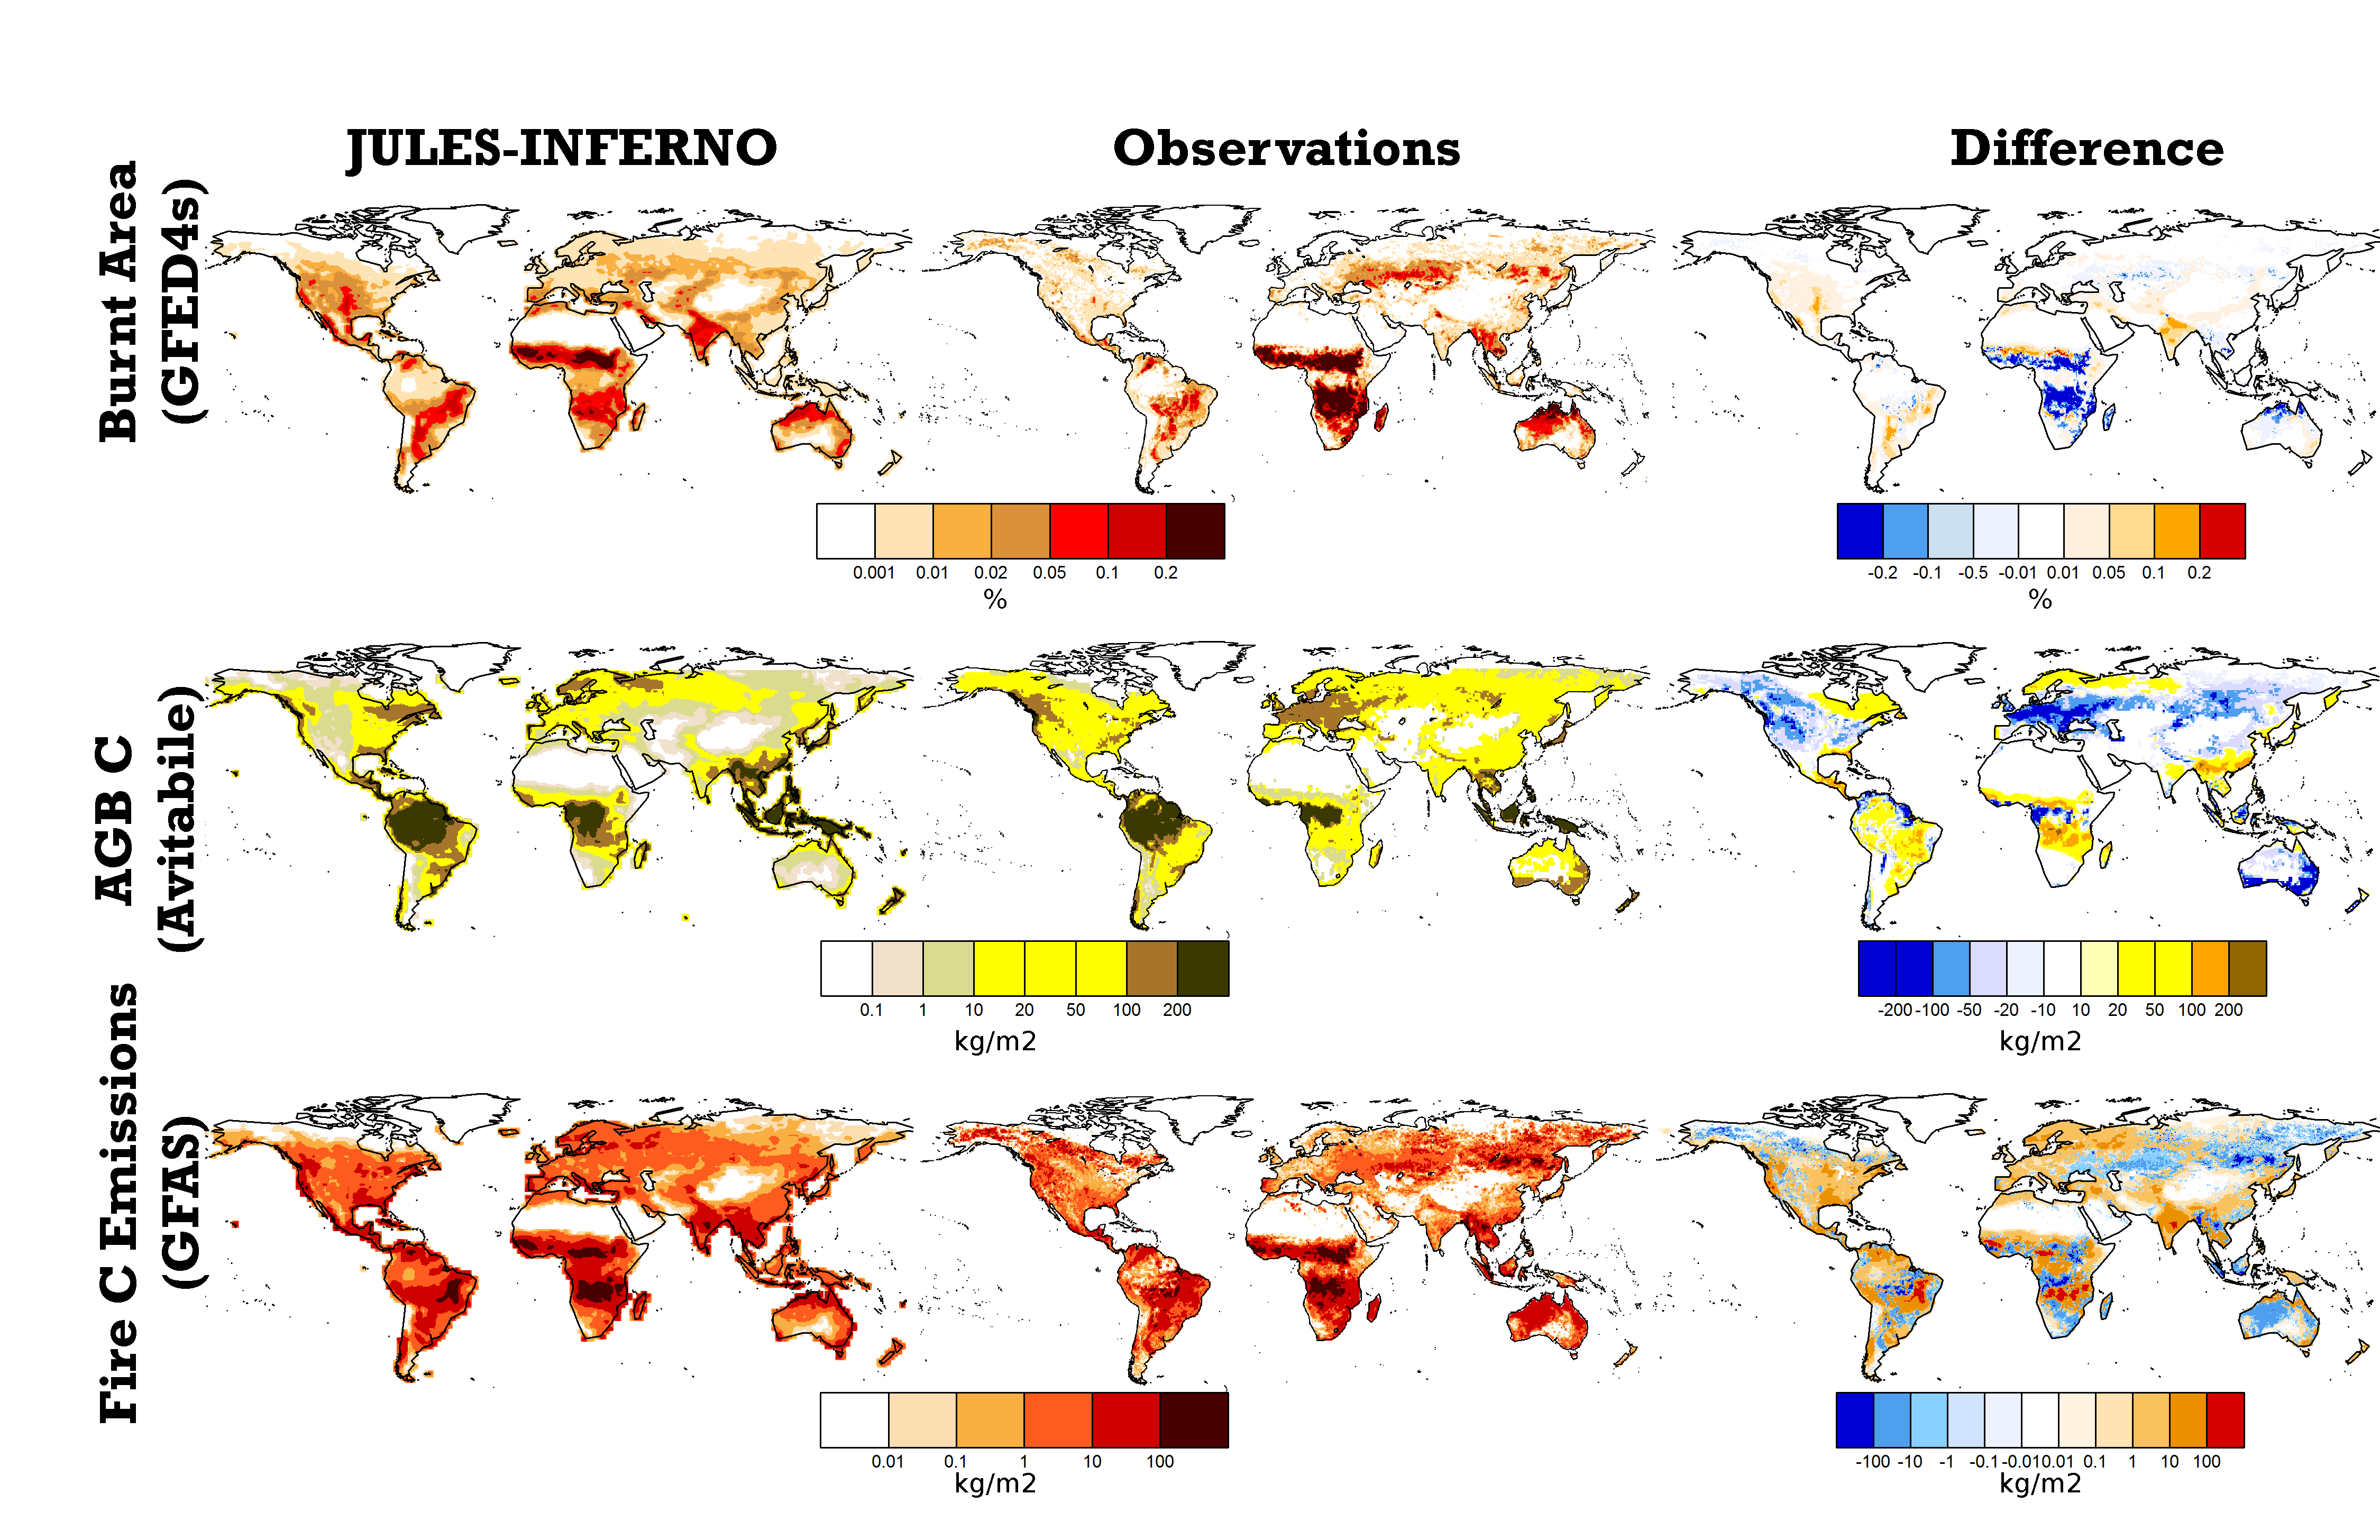
\includegraphics[width=10cm]{images/julesPerformance/FireMapsSpatial.png}
	}
\end{frame}

\begin{frame}[label = kelley2013Datasets]
	\frametitle{Multi-model scores}
	\framesubtitle{Model scores}
	
	\begin{textblock*}{8cm}(11cm ,1.3cm)
		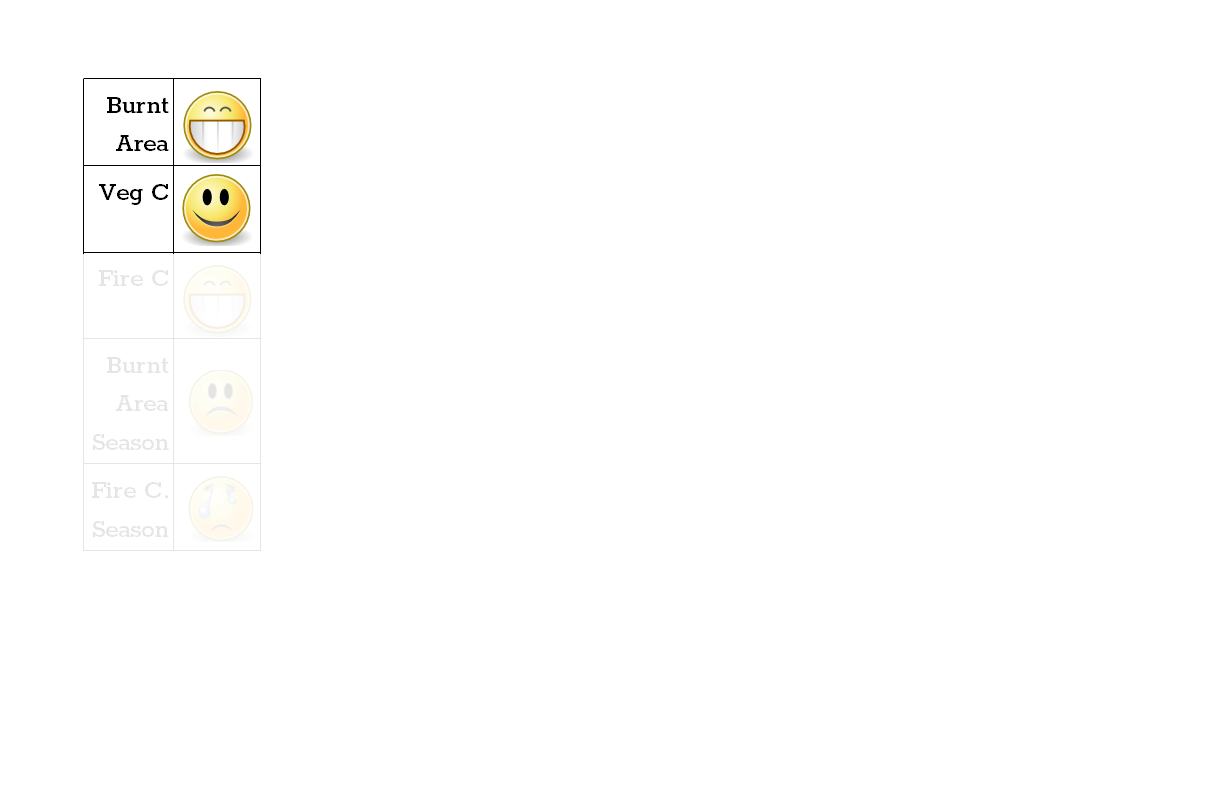
\includegraphics[width=7.5cm]{images/Smileys/BAvegC.png}
	\end{textblock*}
	
	\foreach \x in {1, 2} {
		\only<\x> {
			\includegraphics[width=10cm]{images/fireVsVegScores/pp\x.png}
	}}

\end{frame}



\begin{frame}[label = kelley2013Datasets]
	\frametitle{JULES-INFERNO v obs}
	\framesubtitle{Model scores}
	
	\begin{textblock*}{8cm}(11cm ,1.3cm)
		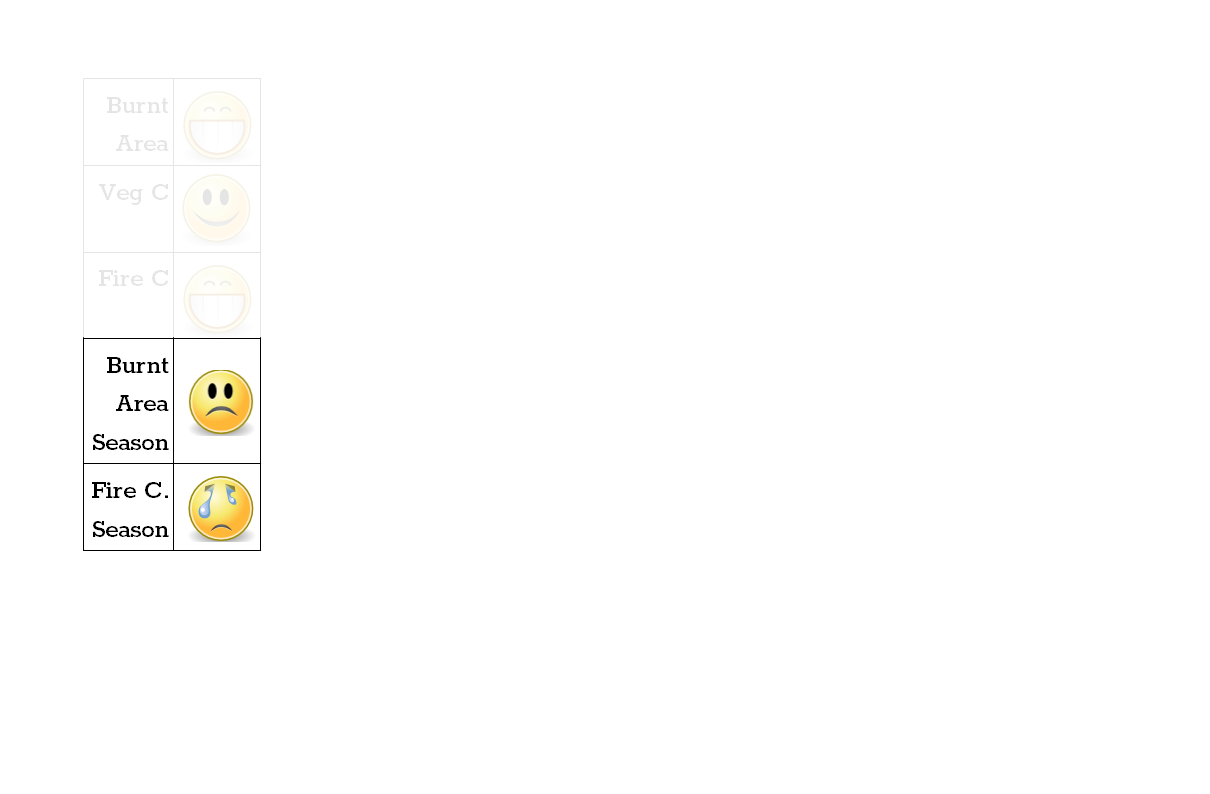
\includegraphics[width=7.5cm]{images/Smileys/BAFireCseason.png}
	\end{textblock*}
	
	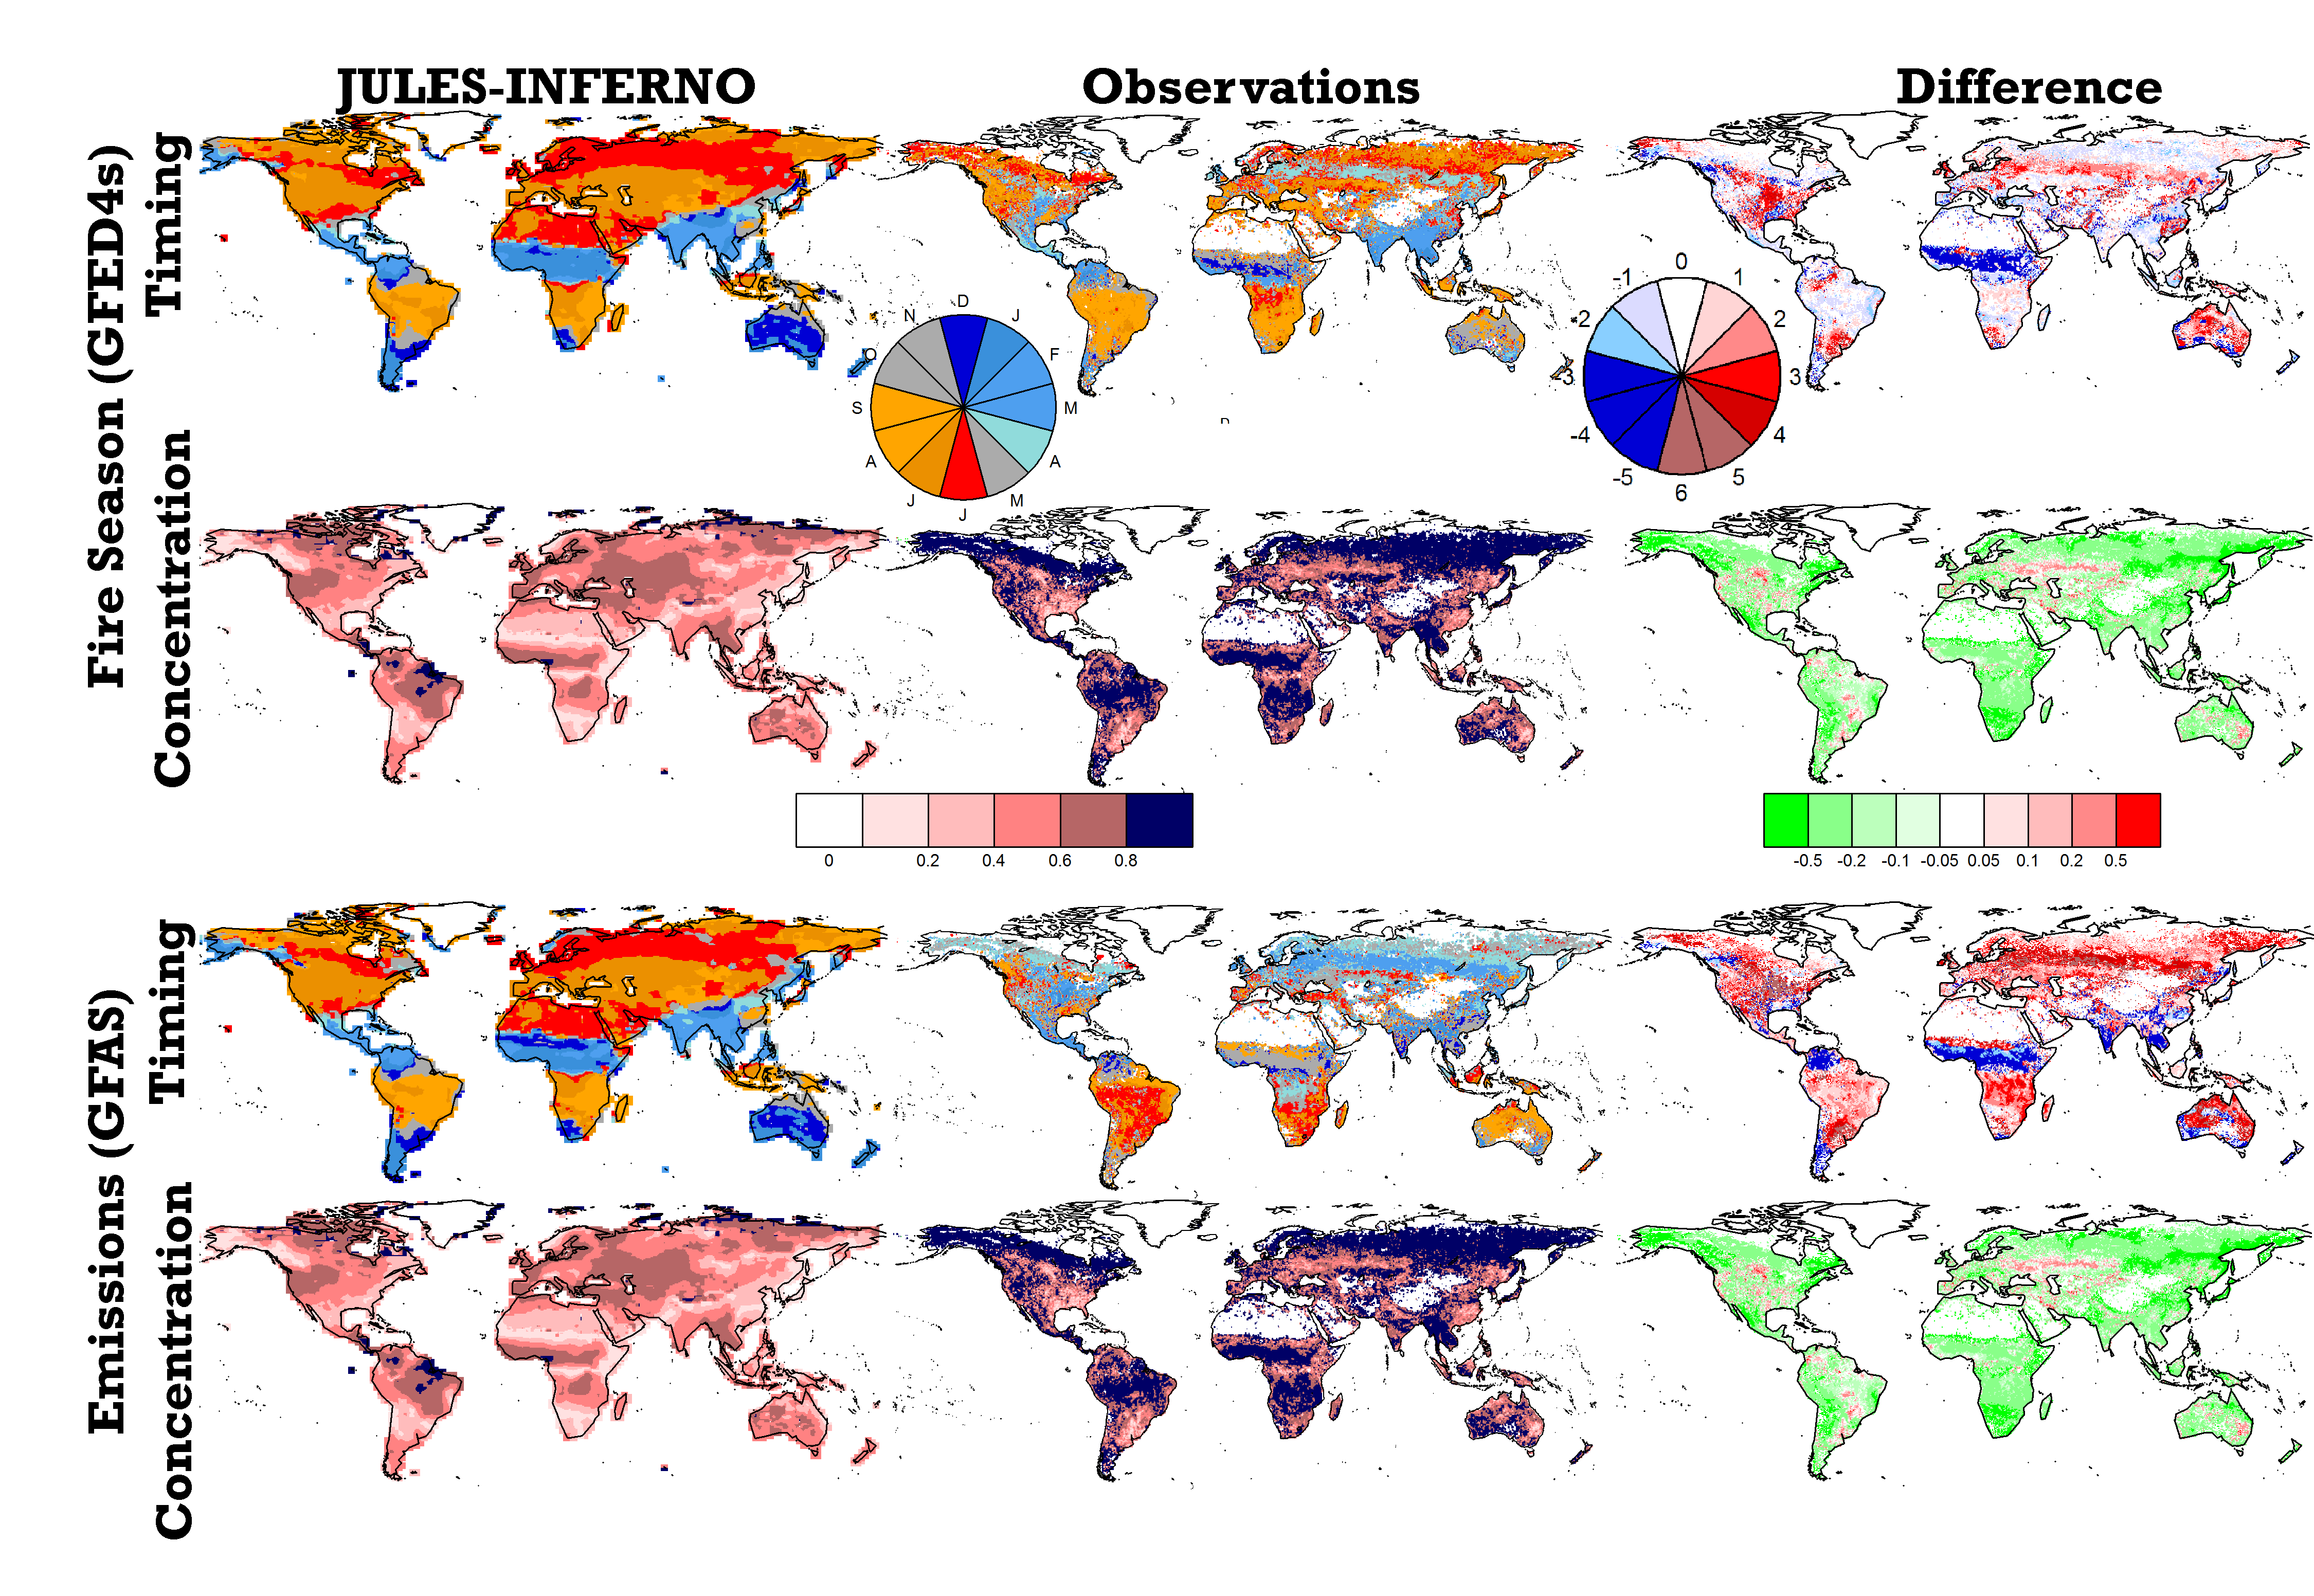
\includegraphics[width=10cm]{images/julesPerformance/FireMapsSeason.png}
	
\end{frame}

%\begin{frame}[label = kelley2013Datasets]
%	\frametitle{Model type scores}
%	\framesubtitle{Model scores}
%	
%	% Model types scores
%\end{frame}

\section{Introduction}
\pgfdeclareimage[width=1.0\paperwidth]{header-image}{header_images/fire2}

\begin{frame}
    \frametitle{It burns where it rains \small{(a bit)}}
    \framesubtitle{Uni-modal relationship with moisture}

	
	\begin{textblock*}{14cm}(-0.5cm,1.5cm)
		\begin{tikzpicture}
	
    \foreach \x in {1, 2, 3, 4, 5} {
        \visible<\x-> {
        
	        \node[anchor=south west,inner sep=0] (image) at (0,0) {
            \includegraphics[width=13.7cm]{images/unimodal/p\x.png}%images/unimodal/p\x.png}
			};}}
			\visible<6-> {
				% Sahel
				\draw[red, line width = 0.25mm] (3.2,5.25) -- (4.0,5.25) -- (4.0,5.4) -- (3.2,5.4) -- (3.2,5.25);
				
				\draw[red, line width = 0.25mm] (3.2,2.05) -- (4.0,2.05) -- (4.0,1.9) -- (3.2,1.9) -- (3.2,2.05);
				
				\draw[red, line width = 0.25mm] (3.6,5.0) -- (4.1,5.0) -- (4.1,4.7) -- (3.6,4.7) -- (3.6,5.0);
				
				\draw[red, line width = 0.25mm] (3.6,1.70) -- (4.1,1.70) -- (4.1,1.4) -- (3.6,1.4) -- (3.6,1.70);
			}
		
			\visible<7-> {
				% India
				\draw[blue, line width = 0.25mm] (4.6,5.2) -- (4.8,5.2) -- (4.8,5.6) -- (4.6,5.6) -- (4.6,5.2);
				
				\draw[blue, line width = 0.25mm] (4.6,1.85) -- (4.8,1.85) -- (4.8,2.25) -- (4.6,2.25) -- (4.6,1.85);
				
				\draw[blue, line width = 0.25mm] (5.6,4.5) -- (5.8,4.4) -- (6.0,4.7) -- (5.8,4.8) -- (5.6,4.5);
				
				\draw[blue, line width = 0.25mm] (5.6,1.15) -- (5.8,1.05) -- (6.0,1.35) -- (5.8,1.45) -- (5.6,1.15);
			}
		    \end{tikzpicture}
    \end{textblock*}
    
    %Make clear we are talking about burnt area
\end{frame}



\begin{frame}[label = intro]
    \frametitle{What else controls fire?}
    %\framesubtitle{Is it Ignitions? Is it people?}
	\begin{itemize}
		\huge{
			\visible<1->{\item \hspace{2.39em}Is it ignitions?}
			\visible<2->{\item If so, Is it people or natural?}
			\visible<3->{\item \hspace{0.70em}Or, Is it something else?}
		}
	\end{itemize}
\hspace{1.5cm} \only<4>{ (it's something else)}
\visible<5->{(it's human suppression)}

\end{frame}


%\begin{frame}
%    \frametitle{What else controls fire?}
%    \framesubtitle{Fire-limitation framework}
%	\begin{itemize}
%		\visible<2-> {\item Map the limitation and sensitivity of burnt area to}
%        \begin{itemize}
%            \visible<3-> {\item Fuel discontinuity}
%            \visible<4-> {\item Fuel moisture and atmospheric drying potential}
%            \visible<5-> {\item lightning and human ignitions}
%            \visible<6-> {\item land use and human suppression}
%        \end{itemize}00
%		\visible<7-> {\item Controls are described from remote sensed and meteorological observations}
%		\visible<8-> {\item optimized againstburnt area observations}00
%	\end{itemize}
%\end{frame}

%\section{Human Impact}

\pgfdeclareimage[width=1.0\paperwidth]{header-image}{header_images/firefighter}


%\begin{frame}
%	\frametitle{INFERNO Fire Controls}
	%\framesubtitle{Geographic controls}
%	\only<1->{
%		\begin{textblock*}{14cm}(0.3cm,5cm)
%			JULES-INFERNO \newline
%			\includegraphics[width=4.8cm]{../../figs/noNothing-INFERNO.png}	
%		\end{textblock*}
%	}
%	
%
%	\only<1->{
%		\begin{textblock*}{14cm}(6.3cm,5cm)
%			Fire Limitation Project (Kelley et al. In prep) \newline
%			\includegraphics[width=4.8cm]{images/igntitions/IgntionInfoNoHumans.png}	
%		\end{textblock*}
%	}
	%\only<3->{
		%\begin{textblock*}{14cm}(6.3cm,6.5cm)
		%	\includegraphics[width=4.8cm]{../../figs/noLand-INFERNO.png}		
		%\end{textblock*}
	%}
	%\begin{textblock*}{14cm}(6.5cm,5.3cm)
	%	\includegraphics[width=5.78cm]{../diagrams/Logistic_fun.png}		
	%\end{textblock*}
%\end{frame}

\begin{frame}
	\frametitle{Human Impact}
	%\framesubtitle{Geographic controls}
	
	\foreach \x in {1, 2, 3, 4} {
		\only<\x> {
			\includegraphics[width=10cm]{images/julesPerformance/Humans\x.png}
	}}
\end{frame} % Model type scores. LimFire etc. Agriculture as a missing process.
\section{Conclusion}

\pgfdeclareimage[width=1.0\paperwidth]{header-image}{header_images/post_fire}

\begin{frame}
    \frametitle{Some things to work on...}
    \framesubtitle{Areas for JULES-INFERNO to improve on}
    
    \begin{textblock*}{8cm}(11cm ,1.3cm)
    	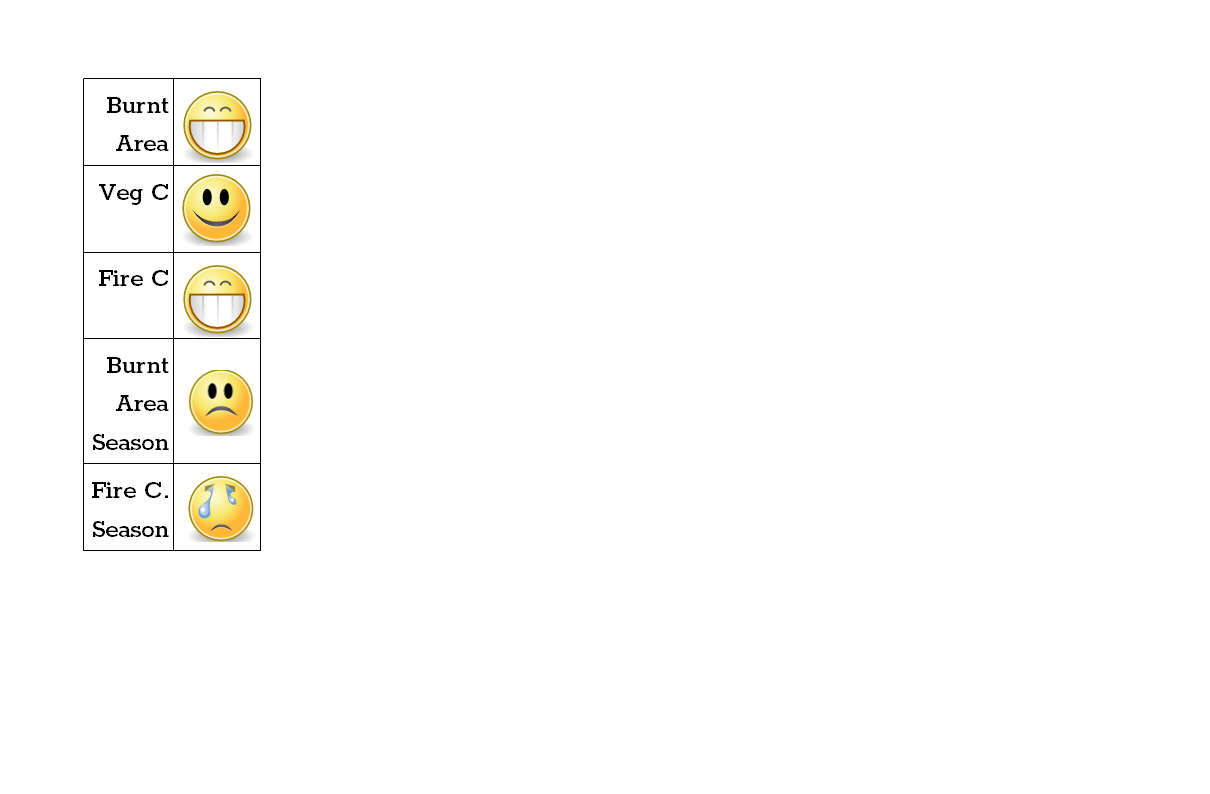
\includegraphics[width=7.5cm]{images/Smileys/All.png}
    \end{textblock*}
    
	\begin{itemize}
		\large{
			\item Burnt area in seasonal humid areas.
			\item Delay fire season onset
			\item Include land use fragmentation
		}
	\end{itemize}
	%\visible<2->{
	%	
	%	\framesubtitle{Other things we could test}
	%	\begin{itemize}
	%		\large{
	%		    \item INFERNO ``offline'' to test impact of veg model coupling (specially on moisture)
	%			\item UKESM-JULES to test impact on simulated climate
	%			\item Some way to test Seasonality problem
	%		}
	%	\end{itemize}
	%}
\end{frame}

\begin{frame}[label = intro]
	\frametitle{fireMIP}
	\framesubtitle{Fire Modelling Inter-comparison Project}
	\begin{textblock*}{14cm}(-0.0cm ,1cm)
		\only<2-> {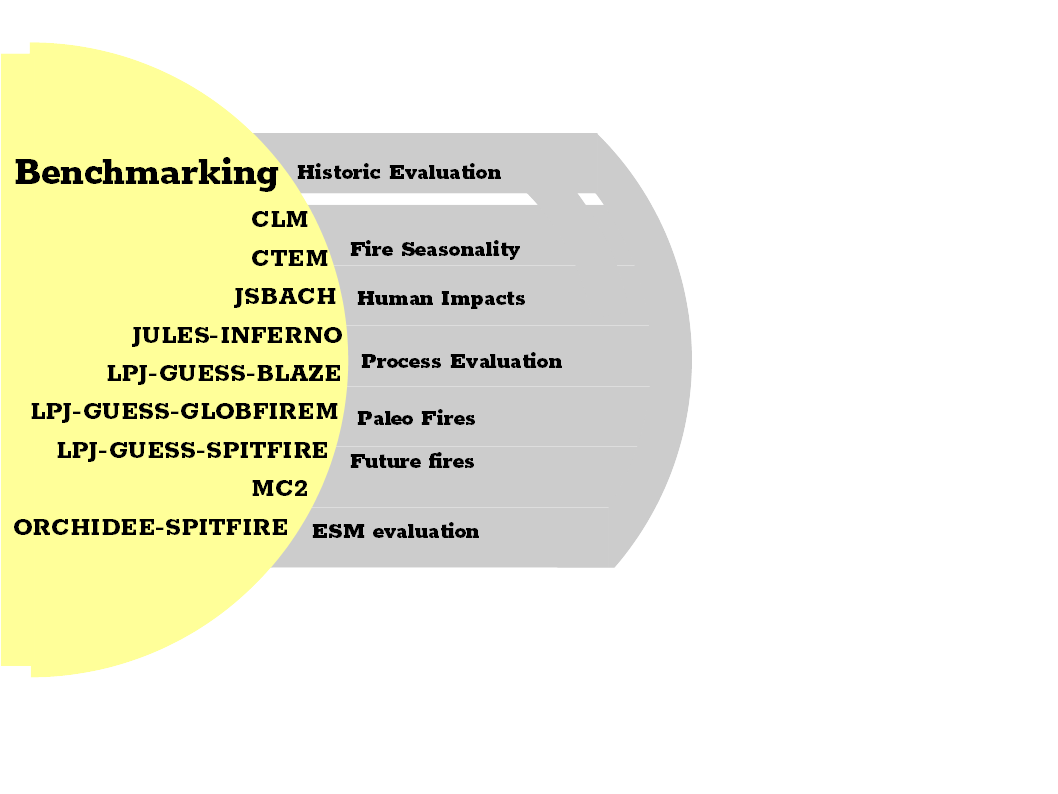
\includegraphics[width=11.7cm]{images/fireMIP/pp-grey.png}}
	\end{textblock*}
	\begin{textblock*}{14cm}(-0.0cm ,1cm)
		%\begin{tikzpicture}
	
				%				\node[anchor=south west,inner sep=0] (image) at (0,0) {
				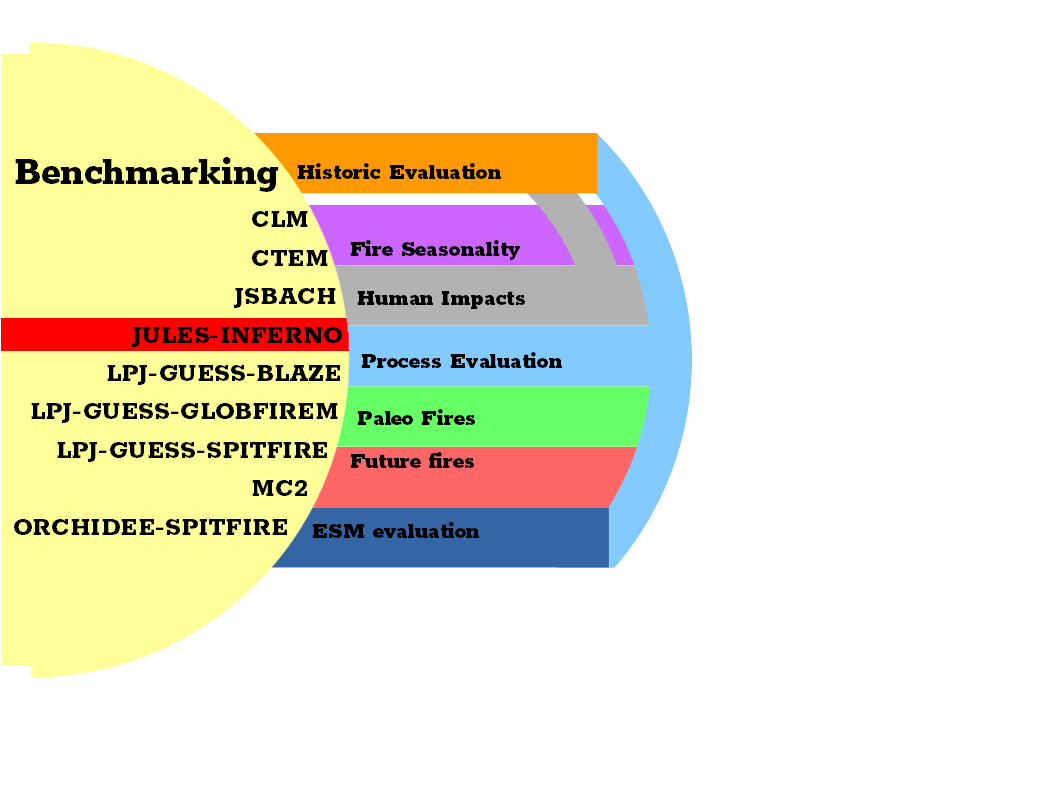
\includegraphics[width=11.7cm]{images/fireMIP/pp5.png}
				%				};
			
		
	\end{textblock*}
	\begin{textblock*}{5.5cm}(7.2cm ,2.5cm)
		%		\node[anchor=south west,inner sep=0] (image) at (6.5cm,0cm) {
		\begin{itemize}
			\small{
			\item World without fire. 
			\item Pre-industrial fire regime. 
			\item Pre-industrial atmospheric CO2. 
			\item Fixed 1700 human population density.
			\item Fixed 1901-1920 lightning. 
			\item Fixed 1901-1920 climate.
			\item Fixed 1700 land use.}
		\end{itemize}
		%		};
		%	\end{tikzpicture}
	\end{textblock*}
	
	%	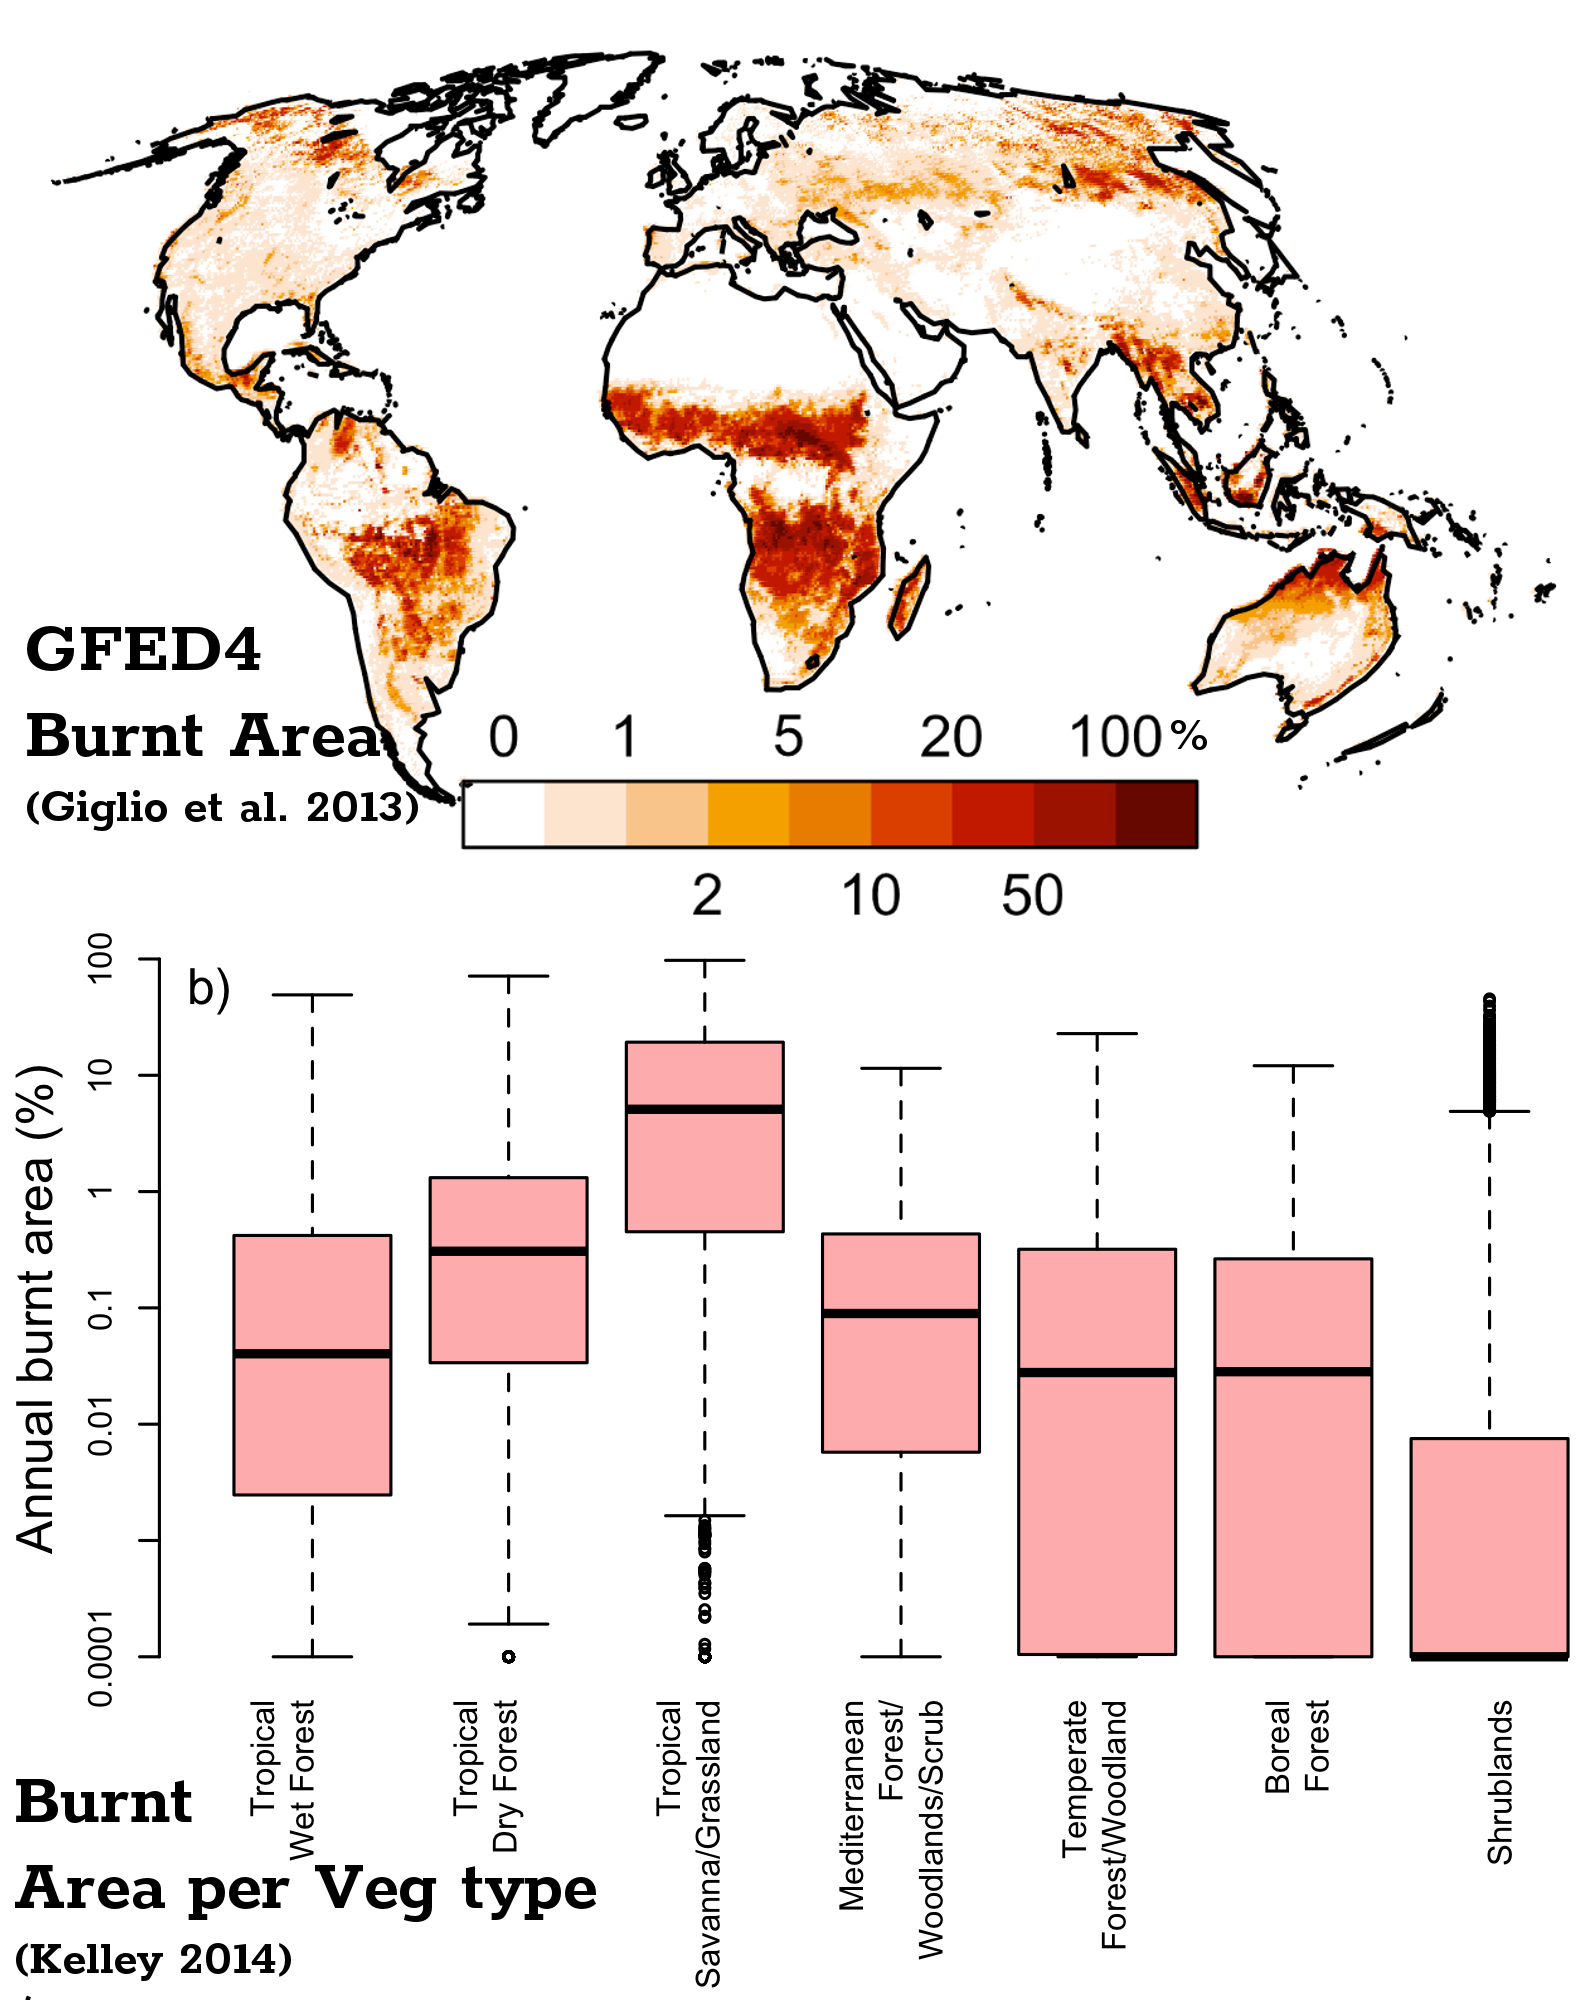
\includegraphics[width=6.05cm]{images/firePerBiome}%images/unimodal/p\x.png}
	%};
	%}}
\end{frame}



%\begin{frame}
%    \frametitle{Questions and suggestion..?}
%    \begin{itemize}
%    	\huge{
%    		\item douglas.i.kelley@gmail.com
%    		\item UKESM-FIRE: tomorrow, 2:30pm 
%    	}
%    \end{itemize}
%\end{frame}
\begin{frame}
    \frametitle{Post-fire recovery}
    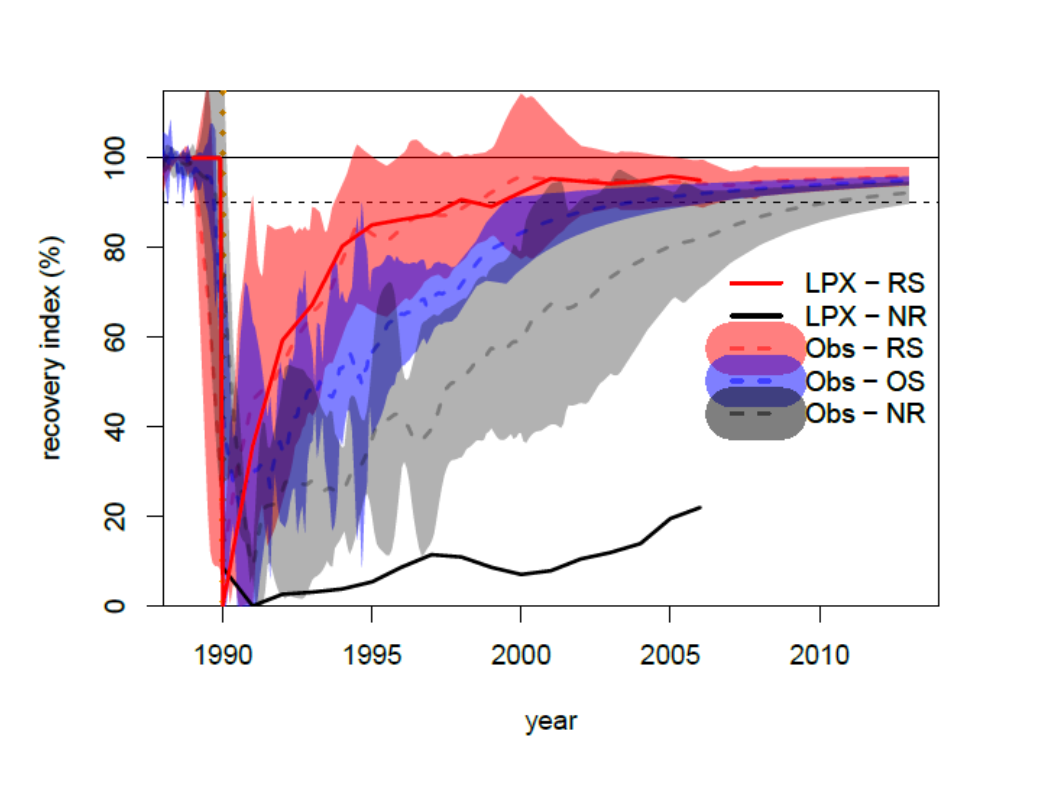
\includegraphics[width=12cm]{images/post-fireRec}%images/unimodal/p\x.png}
\end{frame}


\begin{frame}
	\frametitle{Pre-fire resilience}
	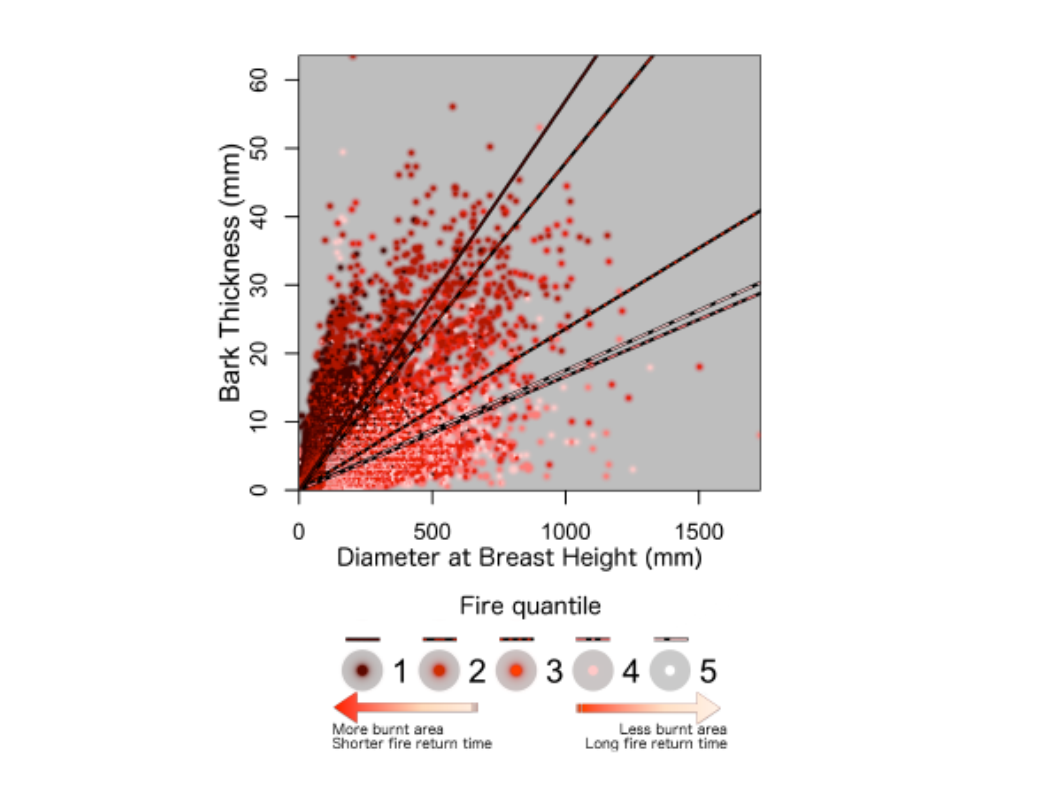
\includegraphics[width=12cm]{images/BTvsDBH}%images/unimodal/p\x.png}
\end{frame}


%\section{Ignitions}
\pgfdeclareimage[width=1.0\paperwidth]{header-image}{header_images/red_lightn}

\begin{frame}<1-3>
    \frametitle{Ignitions}
    \framesubtitle{Humans and Natural \textless Humans + Natural}

	\begin{textblock*}{12cm}(0cm,1.5cm)
    \begin{tikzpicture}
        \node[anchor=south west,inner sep=0] (image) at (0,0) {
            \includegraphics[width=12.0cm]{images/igntitions/IgntionInfoSourceAdding}
        };

        \visible<-1> {\draw[white, fill = white] (6.0,4.4) -- (12.0,4.4) -- (12.0,7.4) -- (6.0,7.4) -- (6.0,4.4);}
        \visible<-2> {\draw[white, fill = white] (0.0,1.0) -- (12.0,1.0) -- (12.0,4.5) -- (0.0,4.5) -- (0.0,1.0);}
    \end{tikzpicture}
	\end{textblock*}
\end{frame}



%\section{Fragmentation}

\pgfdeclareimage[width=1.0\paperwidth]{header-image}{header_images/helicopter}
\againframe<6->{framework}


\begin{frame}
	\frametitle{Controls on fire}
	%\framesubtitle{Geographic controls}
	\begin{textblock*}{14cm}(0.3cm,1.2cm)
		\includegraphics[width=5.78cm]{images/limitCurves/NPPVsFire}	
	\end{textblock*}
	\begin{textblock*}{14cm}(6.5cm,1.2cm)
		\includegraphics[width=5.78cm]{images/limitCurves/alphaVsFire}	
	\end{textblock*}
	\begin{textblock*}{14cm}(0.32cm,5cm)
		\includegraphics[width=5.78cm]{images/limitCurves/ignitionsVsFire.png}		
	\end{textblock*}
	\begin{textblock*}{14cm}(6.5cm,5cm)
		\includegraphics[width=5.78cm]{images/limitCurves/supressionVsFire.png}		
	\end{textblock*}
\end{frame}

\begin{frame}<2>[label=controlMaps]
    \frametitle{So Humans have no impact on fire?}
    \framesubtitle{Suppression \& Fragmentation}
    \controlsSide{limitation_map_no_supression_light}
\end{frame}

\addtocounter{framenumber}{-1}
\begin{frame}<2>[label=controlMaps]
	\frametitle{So Humans have no impact on fire?}
	\framesubtitle{Suppression \& Fragmentation}
	\controlsSide{limitation_map_light}
\end{frame}

\addtocounter{framenumber}{-1}
\begin{frame}<2>[label=controlMaps]
	\frametitle{So Humans have no impact on fire?}
	\framesubtitle{Suppression \& Fragmentation}
	\controlsSide{limitation_map_noColour}
\end{frame}

\addtocounter{framenumber}{-1}
\begin{frame}<2-4>[label=controlMaps]
	\frametitle{So Humans have no impact on fire?}
	\framesubtitle{Suppression \& Fragmentation}
	\controlsSide{limitation_map_light}
	
	\begin{textblock*}{14cm}(3.1cm,3.25cm)
		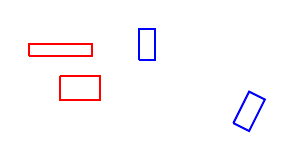
\begin{tikzpicture}
		\visible<5> {
			% Sahel
			\draw[red, line width = 0.25mm] (3.2,5.25) -- (4.0,5.25) -- (4.0,5.4) -- (3.2,5.4) -- (3.2,5.25);
			
			\draw[red, line width = 0.25mm] (3.6,5.0) -- (4.1,5.0) -- (4.1,4.7) -- (3.6,4.7) -- (3.6,5.0);
		}
		\visible<3-> {
			\draw[blue, line width = 0.25mm] (4.6,5.2) -- (4.8,5.2) -- (4.8,5.6) -- (4.6,5.6) -- (4.6,5.2);
			
			\draw[blue, line width = 0.25mm] (5.8,4.4) -- (6.0,4.3) -- (6.2,4.7) -- (6.0,4.8) -- (5.8,4.4);
		}
		\end{tikzpicture}
	\end{textblock*}
	\begin{textblock*}{14cm}(6.7cm,1.45cm)
		
		\only<3>{
			\includegraphics[width=5.7cm]{images/caseStudy/seasonal_casestudyAsia1}}
		\only<4>{
			\includegraphics[width=5.7cm]{images/caseStudy/seasonal_casestudyAsia2}}
	\end{textblock*}
	
\end{frame}



\pgfdeclareimage[width=1.0\paperwidth]{header-image}{header_images/Mirador_de_Garbi}
\begin{frame}
    \frametitle{So Humans have no impact on fire?}
    \framesubtitle{Suppression \& Fragmentation}
    \begin{textblock*}{11cm}(0cm,1.5cm)
    \visible<1->{
    	\begin{tikzpicture}
    	\node[anchor=north,inner sep=0] (image) at (0,0) {
    		\includegraphics[trim={5.1cm 2cm 5.1cm 6.2cm},clip,width=6.2cm]{images/igntitions/IgntionInfoSourceAdding}
	    };
        \node[anchor=south,align=center] at (0, -0.2) {Human Ignitions};
        \end{tikzpicture}
    }
	%trim = {l b r t}
    \visible<1->{
    	\begin{tikzpicture}
    	\node[anchor=north,inner sep=0] (image) at (0,0) {
    		\includegraphics[trim={0 0 0 8cm},clip,width=6.2cm]{images/igntitions/IgntionInfoNoHumans}
    	};
    	\node[anchor=south,align=center] at (0, -0.2) {Overall Human Impact};
    	\end{tikzpicture}
        
    }
    \end{textblock*}
    \begin{textblock*}{11cm}(6.4cm,1.3cm)
    \visible<2->{
        \includegraphics[width=5.5cm]{images/human_noHuman_impact}
    }
    \end{textblock*}

    %\visible<3->{
    %    \begin{tikzpicture}
    %        \node[anchor=south west,inner sep=0] (image) at (0,0) {
    %            \includegraphics[trim={0 0 0 8cm},clip,width=11.0cm]{images/igntitions/IgntionInfoNoHumans}
    %        };
    %
            %\visible<-1> {\draw[white, fill = white] (5.5,4) -- (12.0,4) -- (12.0,0.0) -- (5.5,0.0) -- (5.5,4);}
    %    \end{tikzpicture}
    %}
\end{frame}

\pgfdeclareimage[width=1.0\paperwidth]{header-image}{header_images/firefighter}

%\begin{frame}<2-3>
%    \frametitle{Sensitivity to Controls}
%    \controlsSide{limitation_map}
%\end{frame}

%\section{Conclusion}

\pgfdeclareimage[width=1.0\paperwidth]{header-image}{header_images/post_fire}

\begin{frame}
    \frametitle{Some things to work on...}
    \framesubtitle{Areas for JULES-INFERNO to improve on}
    
    \begin{textblock*}{8cm}(11cm ,1.3cm)
    	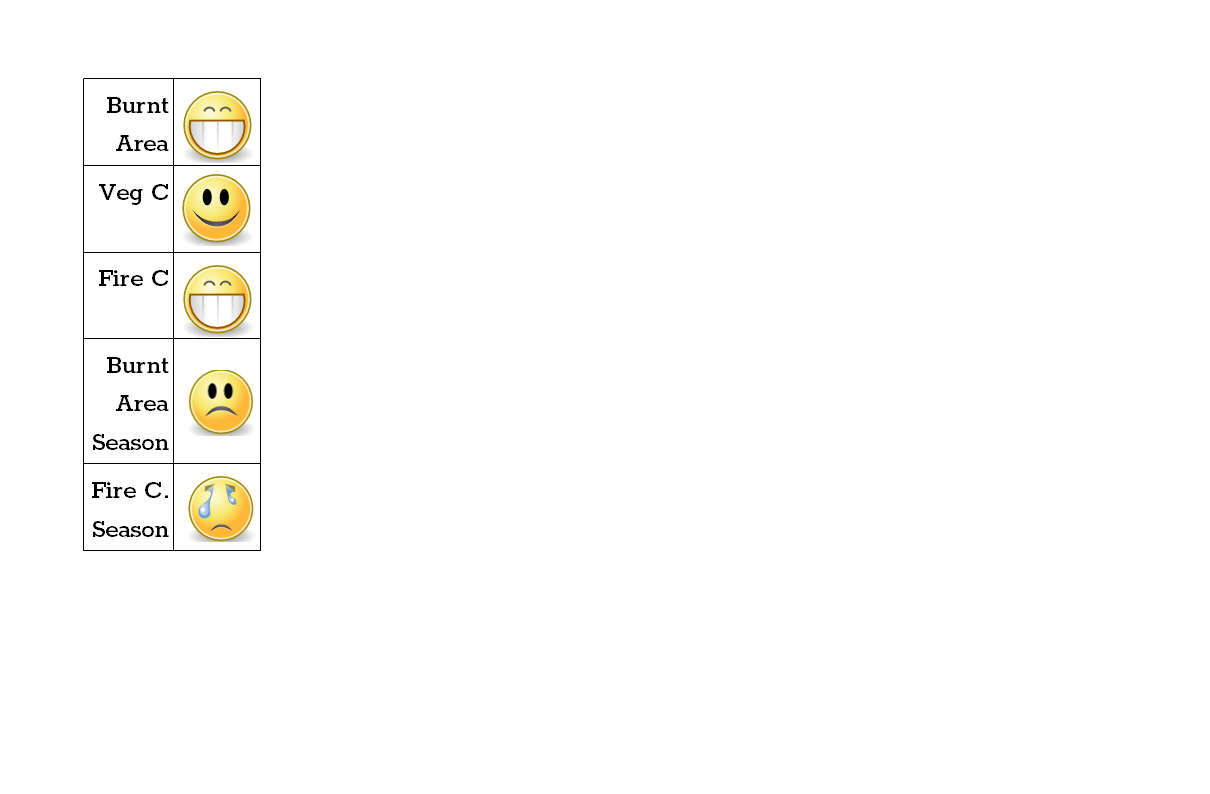
\includegraphics[width=7.5cm]{images/Smileys/All.png}
    \end{textblock*}
    
	\begin{itemize}
		\large{
			\item Burnt area in seasonal humid areas.
			\item Delay fire season onset
			\item Include land use fragmentation
		}
	\end{itemize}
	%\visible<2->{
	%	
	%	\framesubtitle{Other things we could test}
	%	\begin{itemize}
	%		\large{
	%		    \item INFERNO ``offline'' to test impact of veg model coupling (specially on moisture)
	%			\item UKESM-JULES to test impact on simulated climate
	%			\item Some way to test Seasonality problem
	%		}
	%	\end{itemize}
	%}
\end{frame}

\begin{frame}[label = intro]
	\frametitle{fireMIP}
	\framesubtitle{Fire Modelling Inter-comparison Project}
	\begin{textblock*}{14cm}(-0.0cm ,1cm)
		\only<2-> {\includegraphics[width=11.7cm]{images/fireMIP/pp-grey.png}}
	\end{textblock*}
	\begin{textblock*}{14cm}(-0.0cm ,1cm)
		%\begin{tikzpicture}
	
				%				\node[anchor=south west,inner sep=0] (image) at (0,0) {
				\includegraphics[width=11.7cm]{images/fireMIP/pp5.png}
				%				};
			
		
	\end{textblock*}
	\begin{textblock*}{5.5cm}(7.2cm ,2.5cm)
		%		\node[anchor=south west,inner sep=0] (image) at (6.5cm,0cm) {
		\begin{itemize}
			\small{
			\item World without fire. 
			\item Pre-industrial fire regime. 
			\item Pre-industrial atmospheric CO2. 
			\item Fixed 1700 human population density.
			\item Fixed 1901-1920 lightning. 
			\item Fixed 1901-1920 climate.
			\item Fixed 1700 land use.}
		\end{itemize}
		%		};
		%	\end{tikzpicture}
	\end{textblock*}
	
	%	\includegraphics[width=6.05cm]{images/firePerBiome}%images/unimodal/p\x.png}
	%};
	%}}
\end{frame}



%\begin{frame}
%    \frametitle{Questions and suggestion..?}
%    \begin{itemize}
%    	\huge{
%    		\item douglas.i.kelley@gmail.com
%    		\item UKESM-FIRE: tomorrow, 2:30pm 
%    	}
%    \end{itemize}
%\end{frame}
\begin{frame}
    \frametitle{Post-fire recovery}
    \includegraphics[width=12cm]{images/post-fireRec}%images/unimodal/p\x.png}
\end{frame}


\begin{frame}
	\frametitle{Pre-fire resilience}
	\includegraphics[width=12cm]{images/BTvsDBH}%images/unimodal/p\x.png}
\end{frame}

%\section{Example slides}

\begin{frame}
  \frametitle{Prerequisites \& Goals}
  \framesubtitle{Knowledge is a brick wall that you raise line by line forever}
  \begin{block}{LaTeX}
  \begin{itemize}
    \item Obviously some basic LaTeX knowledge is necessary
    \item Some more features will be provided here
  \end{itemize}
  \end{block}

  \begin{block}{Beamer}
  \begin{itemize}
    \item You'll learn them by looking at this presentation source
  \end{itemize}
  \end{block}

  \begin{block}{Goal}
  \begin{itemize}
    \item Learn how to make well structured slides
    \item Using a beautiful theme (congrats to the Oxygen team!)
    \item Take over the world
    \item Relax...
  \end{itemize}
  \end{block}
\end{frame}

\section{Basic structuring}
\begin{frame}
  \frametitle{Sections, Frames and Blocks}
  \framesubtitle{Put everything into boxes}

  The current section is "Basic structuring". And the current frame
  is what you have on the screen right now.

  \begin{block}{A beautiful block}
  A block has a title, and some content. You can put in a block
  almost everything you want that is provided by LaTeX. For example
  math works as usual:
    \begin{equation}
    \sum_{i=1}^n i = \frac{n \times (n+1)}{2}
    \end{equation}
  \end{block}

  Also works outside a block:
  \begin{equation}
  \sum_{i=1}^n i^2 = \frac{n \times (n+1) \times (2n+1)}{6}
  \end{equation}
\end{frame}

\begin{frame}
  \frametitle{Different type of blocks}
  \framesubtitle{Weeeee! Colors!!}
  \begin{block}{Standard block}
  \begin{itemize}
    \item A standard block, used for grouping
    \item Obviously can contain itemizes too...
    \begin{itemize}
      \item And nested itemizes...
      \item of course!
    \end{itemize}
  \end{itemize}
  \end{block}
  \begin{alertblock}{Alert block}
  WARNING: Something very important inside this block!
  \end{alertblock}
  \begin{example}
  Note that examples are displayed as a special block...
  \end{example}
\end{frame}

\section{Fancy features}
\begin{frame}
  \frametitle{Highlighting}
  \framesubtitle{Hey! Look here! here!}

  \begin{block}{A regular block}
  \begin{itemize}
    \item Normal text
    \item \highlighton{Highlighted text} to draw attention
    \item \alert{"Alert'ed" text} to spot very important information
    \item Alternatively you can
    \begin{itemize}
      \alert{\item "Alert" the item itself}
      \highlighton{\item Or "Highlight" it}
    \end{itemize}
  \end{itemize}
  \end{block}
  \begin{alertblock}{If it's very very important...}
  \alert{... you can "alert" in an "alertblock"}\\
  Ewww, nasty, heh?
  \end{alertblock}
\end{frame}

\newcommand{\putlink}[1]{%
   \pgfsetlinewidth{1.4pt}%
   \pgfsetendarrow{\pgfarrowtriangle{4pt}}%
   \pgfline{\pgfxy(1,1)}{\pgfxy(#1,1)}
}

\begin{frame}
  \frametitle{Overlay effects}
  \framesubtitle{Keep the suspense!}
  \begin{block}{Time bomb}
  \begin{enumerate}
    \item<2-> Two more to go
    \item<3-> One more to go
    \item<4-> Last chance...
    \item<5-> BOOM!
  \end{enumerate}
  \end{block}
  \begin{block}{"Animation"}<6->
    \begin{pgfpicture}{0cm}{0cm}{7cm}{2cm}
    \only<1-6>{
      \putlink{2}
    }
    \only<7>{
      \putlink{4}
    }
    \only<8>{
      \putlink{6}
    }
    \only<9>{
      \putlink{8}
    }
    \only<10>{
      \putlink{10}
    }
    \end{pgfpicture}
  \end{block}
\end{frame}

\section*{}
\frame{
  \vfill
  \centering
  \highlighton{
  \usebeamerfont*{frametitle}And now?

  \usebeamerfont*{framesubtitle}Enter the secret section
  }
  \vfill
}
\begin{frame}
  \frametitle{Contributing to this beamer style}
  \framesubtitle{We want you !}

  \begin{block}{Why?}
  \begin{itemize}
    \item Beamer is hot!
    \item This style deserves to be improved
  \end{itemize}
  \end{block}

  \begin{block}{How?}
  \begin{itemize}
    \item Grab it
    \item Improve its LaTeX code
    \item Use you artistics skills
    \item Document it
    \item Help other people to use it
    \item Use it...
  \end{itemize}
  \end{block}
\end{frame}

\begin{frame}
  \frametitle{Resources}
  \framesubtitle{If you want to improve this style}
  \begin{thebibliography}{10}

  \beamertemplatearticlebibitems

  \bibitem{beamer-homepage}
    LaTeX Beamer
    \newblock {\tt http://latex-beamer.sourceforge.net/}

  \bibitem{kdeslides}
    KDE Presentations
    \newblock {\tt http://www.kde.org/kdeslides/}

  \end{thebibliography}
\end{frame}

\frame{
  \vspace{2cm}
  {\huge Questions ?}

  \vspace{3cm}
  \begin{flushright}
    Konqi Konqueror

    \structure{\footnotesize{konqi@kde.org}}
  \end{flushright}
}


\end{document}
